\documentclass{tufte-book}

\hypersetup{colorlinks}% uncomment this line if you prefer colored hyperlinks (e.g., for onscreen viewing)

%%
% Book metadata
%\title{CCD instruments and calibration}
\title{PHYC40870\\
Space Detector\\
Laboratory}
%\author[The Tufte-LaTeX Developers]{The Tufte-LaTeX\ Developers}
\publisher{MSc Space Science}

%%
% If they're installed, use Bergamo and Chantilly from www.fontsite.com.
% They're clones of Bembo and Gill Sans, respectively.
%\IfFileExists{bergamo.sty}{\usepackage[osf]{bergamo}}{}% Bembo
%\IfFileExists{chantill.sty}{\usepackage{chantill}}{}% Gill Sans

%\usepackage{microtype}

%%
% Just some sample text
\usepackage{lipsum}
\usepackage{tcolorbox} 
\PassOptionsToPackage{hyphens}{url}
\usepackage{hyperref}
 
\newsavebox\myboxA
\newsavebox\myboxB
\newlength\mylenA

\newcommand*\xoverline[2][0.75]{%
    \sbox{\myboxA}{$\m@th#2$}%
    \setbox\myboxB\null% Phantom box
    \ht\myboxB=\ht\myboxA%
    \dp\myboxB=\dp\myboxA%
    \wd\myboxB=#1\wd\myboxA% Scale phantom
    \sbox\myboxB{$\m@th\overline{\copy\myboxB}$}%  Overlined phantom
    \setlength\mylenA{\the\wd\myboxA}%   calc width diff
    \addtolength\mylenA{-\the\wd\myboxB}%
    \ifdim\wd\myboxB<\wd\myboxA%
       \rlap{\hskip 0.5\mylenA\usebox\myboxB}{\usebox\myboxA}%
    \else
        \hskip -0.5\mylenA\rlap{\usebox\myboxA}{\hskip 0.5\mylenA\usebox\myboxB}%
    \fi}


%%
% For nicely typeset tabular material
\usepackage{booktabs}

\usepackage{listings}

%%
% For graphics / images
\usepackage{graphicx}
\setkeys{Gin}{width=\linewidth,totalheight=\textheight,keepaspectratio}
\graphicspath{{graphics/}}

% The fancyvrb package lets us customize the formatting of verbatim
% environments.  We use a slightly smaller font.
\usepackage{fancyvrb}
\fvset{fontsize=\normalsize}

%%
% Prints argument within hanging parentheses (i.e., parentheses that take
% up no horizontal space).  Useful in tabular environments.
\newcommand{\hangp}[1]{\makebox[0pt][r]{(}#1\makebox[0pt][l]{)}}

%%
% Prints an asterisk that takes up no horizontal space.
% Useful in tabular environments.
\newcommand{\hangstar}{\makebox[0pt][l]{*}}

\usepackage{pdfpages}

%%
% Prints a trailing space in a smart way.
\usepackage{xspace}


\newcommand{\TL}{Tufte-\LaTeX\xspace}

% Prints the month name (e.g., January) and the year (e.g., 2008)
\newcommand{\monthyear}{%
  \ifcase\month\or January\or February\or March\or April\or May\or June\or
  July\or August\or September\or October\or November\or
  December\fi\space\number\year
}


% Prints an epigraph and speaker in sans serif, all-caps type.
\newcommand{\openepigraph}[2]{%
  %\sffamily\fontsize{14}{16}\selectfont
  \begin{fullwidth}
  \sffamily\large
  \begin{doublespace}
  \noindent\allcaps{#1}\\% epigraph
  \noindent\allcaps{#2}% author
  \end{doublespace}
  \end{fullwidth}
}

% Inserts a blank page
\newcommand{\blankpage}{\newpage\hbox{}\thispagestyle{empty}\newpage}

\usepackage{units}
\usepackage{amsmath}
% Typesets the font size, leading, and measure in the form of 10/12x26 pc.
\newcommand{\measure}[3]{#1/#2$\times$\unit[#3]{pc}}

% Macros for typesetting the documentation
\newcommand{\hlred}[1]{\textcolor{Maroon}{#1}}% prints in red
\newcommand{\hangleft}[1]{\makebox[0pt][r]{#1}}
\newcommand{\hairsp}{\hspace{1pt}}% hair space
\newcommand{\hquad}{\hskip0.5em\relax}% half quad space
\newcommand{\TODO}{\textcolor{red}{\bf TODO!}\xspace}
\newcommand{\ie}{\textit{i.\hairsp{}e.}\xspace}
\newcommand{\eg}{\textit{e.\hairsp{}g.}\xspace}
\newcommand{\na}{\quad--}% used in tables for N/A cells
\providecommand{\XeLaTeX}{X\lower.5ex\hbox{\kern-0.15em\reflectbox{E}}\kern-0.1em\LaTeX}
\newcommand{\tXeLaTeX}{\XeLaTeX\index{XeLaTeX@\protect\XeLaTeX}}
% \index{\texttt{\textbackslash xyz}@\hangleft{\texttt{\textbackslash}}\texttt{xyz}}
\newcommand{\tuftebs}{\symbol{'134}}% a backslash in tt type in OT1/T1
\newcommand{\doccmdnoindex}[2][]{\texttt{\tuftebs#2}}% command name -- adds backslash automatically (and doesn't add cmd to the index)
\newcommand{\doccmddef}[2][]{%
  \hlred{\texttt{\tuftebs#2}}\label{cmd:#2}%
  \ifthenelse{\isempty{#1}}%
    {% add the command to the index
      \index{#2 command@\protect\hangleft{\texttt{\tuftebs}}\texttt{#2}}% command name
    }%
    {% add the command and package to the index
      \index{#2 command@\protect\hangleft{\texttt{\tuftebs}}\texttt{#2} (\texttt{#1} package)}% command name
      \index{#1 package@\texttt{#1} package}\index{packages!#1@\texttt{#1}}% package name
    }%
}% command name -- adds backslash automatically
\newcommand{\doccmd}[2][]{%
  \texttt{\tuftebs#2}%
  \ifthenelse{\isempty{#1}}%
    {% add the command to the index
      \index{#2 command@\protect\hangleft{\texttt{\tuftebs}}\texttt{#2}}% command name
    }%
    {% add the command and package to the index
      \index{#2 command@\protect\hangleft{\texttt{\tuftebs}}\texttt{#2} (\texttt{#1} package)}% command name
      \index{#1 package@\texttt{#1} package}\index{packages!#1@\texttt{#1}}% package name
    }%
}% command name -- adds backslash automatically
\newcommand{\docopt}[1]{\ensuremath{\langle}\textrm{\textit{#1}}\ensuremath{\rangle}}% optional command argument
\newcommand{\docarg}[1]{\textrm{\textit{#1}}}% (required) command argument
\newenvironment{docspec}{\begin{quotation}\ttfamily\parskip0pt\parindent0pt\ignorespaces}{\end{quotation}}% command specification environment
\newcommand{\docenv}[1]{\texttt{#1}\index{#1 environment@\texttt{#1} environment}\index{environments!#1@\texttt{#1}}}% environment name
\newcommand{\docenvdef}[1]{\hlred{\texttt{#1}}\label{env:#1}\index{#1 environment@\texttt{#1} environment}\index{environments!#1@\texttt{#1}}}% environment name
\newcommand{\docpkg}[1]{\texttt{#1}\index{#1 package@\texttt{#1} package}\index{packages!#1@\texttt{#1}}}% package name
\newcommand{\doccls}[1]{\texttt{#1}}% document class name
\newcommand{\docclsopt}[1]{\texttt{#1}\index{#1 class option@\texttt{#1} class option}\index{class options!#1@\texttt{#1}}}% document class option name
\newcommand{\docclsoptdef}[1]{\hlred{\texttt{#1}}\label{clsopt:#1}\index{#1 class option@\texttt{#1} class option}\index{class options!#1@\texttt{#1}}}% document class option name defined
\newcommand{\docmsg}[2]{\bigskip\begin{fullwidth}\noindent\ttfamily#1\end{fullwidth}\medskip\par\noindent#2}
\newcommand{\docfilehook}[2]{\texttt{#1}\index{file hooks!#2}\index{#1@\texttt{#1}}}
\newcommand{\doccounter}[1]{\texttt{#1}\index{#1 counter@\texttt{#1} counter}}

\usepackage{textgreek}
\newcommand{\alphadecay}{\textalpha}
\newcommand{\betaminus}{\textbeta\textsuperscript{$-$}}
\newcommand{\gammadecay}{\textgamma}

\newcommand{\gmray}{$\gamma$-ray}
% Generates the index
\usepackage{makeidx}
\makeindex

\begin{document}

% Front matter
\frontmatter


% r.3 full title page
\maketitle


% v.4 copyright page
\newpage
\begin{fullwidth}
\vfill
\thispagestyle{empty}
\setlength{\parindent}{0pt}
\setlength{\parskip}{\baselineskip}
%Copyright \copyright\ \the\year\ \thanklessauthor

%\par\smallcaps{Published by \thanklesspublisher}

%\par\smallcaps{tufte-latex.googlecode.com}

\smallcaps{Authors: \\
                    Morgan Fraser (morgan.fraser@ucd.ie, UCD School of Physics)\\
                    Andrew Kirwan (andrew.kirwan1@ucd.ie, UCD School of Physics)}\\
\smallskip
\smallcaps{version 0.1, 28 May 2025}\\


%\noindent\fbox{%
%    \parbox{\textwidth}{%
%      \bf{Important - in light of COVID restrictions I will not be regularly walking around the labs. If you have questions, ideas or want to discuss the  experiment, please e-mail me at the %address above, and we can arrange to either meet in person / discuss on Zoom or by e-mail as necessary.}
      
%    }%
%}



%\par Licensed under the Apache License, Version 2.0 (the ``License''); you may not
%use this file except in compliance with the License. You may obtain a copy
%of the License at \url{http://www.apache.org/licenses/LICENSE-2.0}. Unless
%required by applicable law or agreed to in writing, software distributed
%under the License is distributed on an \smallcaps{``AS IS'' BASIS, WITHOUT
%WARRANTIES OR CONDITIONS OF ANY KIND}, either express or implied. See the
%License for the specific language governing permissions and limitations
%under the License.\index{license}
%
%\par\textit{First printing, \monthyear}
\end{fullwidth}

% r.5 contents
\tableofcontents

%\listoffigures

%\listoftables

% r.7 dedication
%\cleardoublepage
%~\vfill
%\begin{doublespace}
%\noindent\fontsize{18}{22}\selectfont\itshape
%\nohyphenation
%Dedicated to those who appreciate \LaTeX{} 
%and the work of \mbox{Edward R.~Tufte} 
%and \mbox{Donald E.~Knuth}.
%\end{doublespace}
%\vfill
%\vfill


%% r.9 introduction
%\cleardoublepage
%\chapter*{Introduction}
%
%This sample book discusses the design of Edward Tufte's
%books\cite{Tufte2001,Tufte1990,Tufte1997,Tufte2006}
%and the use of the \doccls{tufte-book} and \doccls{tufte-handout} document classes.


%%
% Start the main matter (normal chapters)
\mainmatter


\chapter{Introduction to PHYC40870}
\section{Module Overview}
% Aims of the module, how it is strucutred etc.
% \begin{fullwidth}
    
{The Space Detector Laboratory} is a 10 credit core module for the MSc Space Science \& Technology course. This is a lab-based module with lab sessions scheduled for Mondays and Tuesdays from 14:00-15:00. You will be expected to do independent work, including (but not limited to) preparation, reading, coding, and report writing outside of these hours. 

This module is intended to instill a working, functional understanding of detector systems and imaging technology, as well as provide practical experience with ``CubeSat`` and nano-satellite systems. These skills will prepare you for both the Space Mission Design field trip, and the Satellite Subsystems lab in Semester 2. Additionally, we will introduce you to some essential coding skills in the Python programming language, which will further aid you later in your studies.


The module has three primary components:

\begin{itemize}
    \item CCDs \& Imaging Techniques
    \item Gamma-ray Detectors in Space \& Astronomy
    \item ``AMSAT`` (\textbf{Am}ateur \textbf{Sat}ellite) and CubeSat systems
\end{itemize}

\newpage

% \end{fullwidth}
\section{Course schedule}

order is python > optical > he detectors > amsat. Need to update table below
\begin{table}
    \centering
    \begin{tabular}{c|c|c}
        W1 & Mon 8th Sept & Introduction to Python \\
           & Tue 9th      & Introduction to Python \\
           \hline
        W2 & Mon 15th     & Introduction to Python \\
           & Tues 16th    & GitHub\\
           \hline
        W3 & Mon 22nd     & Virtual environments\\
           & Tues 23rd    & ChatGPT\\
           \hline
        W4 & Mon 29th     & Optical detectors lecture\\
           & Tues 30th    & HST data exercise \\
           \hline
        W5 & Mon 6th Oct  & HST data exercise\\
           & Tues 7th     & Sentinel-2 exercise\\
           \hline
        W6 & Mon  13th    & Sentinel-2 exercise\\
           \hline
        W11 & Mon 17th    & AMSAT - introduction\\
           & Tues 18th    & AMSAT - connecting \\
           \hline
        W12 & Mon 24th    & AMSAT experiments\\
           & Tues 25th    & AMSAT experiments\\
        
           & Tues 14th    & High energy detectors lecture\\
           \hline
        W7 & Mon 20th     & Detector 1 experiment\\
           & Tues 21st    & Detector 1 experiment\\
           \hline
        W8 & Mon 27th     & Public holiday\\
           & Tues 28th    & Detector 1 experiment\\
           \hline
        W9 & Mon 3rd Nov  & Detector 2 experiment\\
           & Tues 4th     & Detector 2 experiment\\
           \hline
        W10 & Mon 10th    & Detector 2 experiment\\
           & Tues 11st    & Merge detector results\\
    \end{tabular}
    \label{tab:my_label}
\end{table}



\newpage

% \end{fullwidth}
\section{Assesment \& Deliverables}

{Throughout} the course you will be assessed through a combination of assignments and continuous assessments. The assessed deliverables are as follows: \textbf{(Andrew's note: just need to figure out weightings for the assessments.)}
% \end{fullwidth}

\begin{enumerate}
    \item Programming in Python
    \begin{itemize}
        \item Code submissions
    \end{itemize}
    \item Optical and Other Detectors
    \begin{itemize}
        \item Code submissions
    \end{itemize}
    \item Gamma-ray Detectors in Astronomy
    \begin{itemize}
        \item Code submissions
        \item Final Report
    \end{itemize}
    \item AMSAT
    \begin{itemize}
        \item Final Report
    \end{itemize}
\end{enumerate}


\chapter{Computing fundamentals}
\label{ch:python}

\section{Python}
\label{sec:python}
\subsection{Why Python?}
\label{subsec:python-intro}

% Why they need to learn Python, some links to good online courses
{Python} is an open-source, easily accessible, and powerful programming and scripting language which has become increasingly popular in a variety of disciplines, particularly astronomy and physics. The most accessible and practical use of the language is with the Raspberry Pi computer and other microcontrollers, as these are especially well-documented by DIY enthusiasts, ``makers'', and electronics hobbyists. We see it used in higher-level situations as well: for example, CubeSats and nano-satellites (which will be discussed later) often have software/hardware interfaces controlled with the Python language, and state-of-the-art telescopes like the James Webb Space Telescope (JWST) feature data reduction pipelines written almost entirely in Python. 

Perhaps most attractive is the simplicity and human-like syntax of the language; this ease of use has made Python a choice language for statistics, machine learning, and data reduction and visualization. Additionally, its popularity has led to the community development of countless tools (called ``modules'' or packages) that can be imported into your workspace and used with minimal effort, preventing the need to ``reinvent the wheel'' when writing your own code for data analysis. Overall it is a user-friendly and easy-to-learn language that offers accessibility to a host of disciplines for both the humble beginner and the seasoned programmer. 

Some of you may have prior experience with Python, though we anticipate that few of you will have experience using it to write more extended software or for interfacing with hardware. In our practical sessions, we will be helping to lay a foundation for your learning in this respect in order to prepare you not only for upcoming modules, but for your future careers as well. To this end we have provided a number of resources for you to utilize throughout the course; as our laboratory time is limited, it is expected that you consult these references outside of our scheduled times, and familiarize yourself with some of the fundamentals prior to our sessions. For ease of reference you can find these supplementary sources at the end of this section.

\subsection{Installation}\label{subsec:python-install}

{There are several ways} to install Python, and the method you choose really depends on what you are most comfortable doing. The easiest method by far is through the Anaconda distribution platform, which has two ``flavors`` or installations from which to choose: \href{http://conda.pydata.org/miniconda.html}{miniconda} and \href{https://www.anaconda.com/download}{anaconda}. Both of these version rely on the same underlying architecture which installs both Python and the command-line tool \verb|conda|. Miniconda is a lightweight version which only installs the bare minimum (that is, \textit{only} Python and \verb|conda|), while Anaconda includes a massive collection of pre-installed packages that are commonly used in scientific computing. 

For this course we recommend the miniconda package. Full details of how to use the architecture can be found on their website. Once it is installed, you can access the Anaconda prompt by using the Windows Start Menu (if you are using Windows). On MacOS or Linux, you can open up a terminal and type \verb|conda activate|. Once you've activated miniconda you should see something like

\begin{lstlisting}[backgroundcolor=\color{lightgray}]
(base) C:\Users\YourUsername>   # for Windows
[...]
(base) user@hostname:-$       # for Mac/Linux
\end{lstlisting}
% \end{lstlisting}

Throughout this handbook, we will present all operations from the command line or terminal in the style:
\begin{lstlisting}[backgroundcolor=\color{lightgray}]
$ [code goes here]
\end{lstlisting}

\subsection{Virtual environments}\label{subsec:python-venv}

{By default}, miniconda will activate the ``base`` environment so you might see \verb|(base)| at the beginning of the command line. Environments are a useful way to keep your installed packages compartmentalized. This is especially important if you're designing some kind of software that other people might want to download and install, as it ensures that all the necessary \textit{dependencies} (the packages that your project depends on to work) are satisfied within that project environment. It also prevents you from accidentally removing a package that your computer might need in order to run, or from adding a different version of a package that might conflict with a similar package on your computer. While the Anaconda ecosystem is generally quite good at handling dependency conflicts, it's still best practice to create a \textit{virtual environment} for your project to keep things clean. 

To create an environment, you can simply open the command terminal and type 

\begin{lstlisting}[backgroundcolor=\color{lightgray}]
$ conda create -n NAME
\end{lstlisting}

The \verb|conda| commands \verb|activate NAME| and \verb|deactivate NAME| will either activate or deactivate an environment you have named \verb|NAME|. You can install packages using the \verb|install| command. For our course, the most useful packages are \texttt{numpy}, \texttt{scipy}, \texttt{matplotlib}, and \texttt{jupyter}. We will discuss packages in more depth shortly.

\begin{tcolorbox}[sharp corners=all, colback=white!75!green]
%[width=\linewidth, sharp corners=all, colback=white!95!black]

Coding Exercise:

Use the \verb|conda| package to create a virtual environment called \verb|spacelab| and install the four packages listed above.

\end{tcolorbox} 


% \begin{tcolorbox}[sharp corners=all, colback=white!75!green]
%[width=\linewidth, sharp corners=all, colback=white!95!black]

% Topics we should cover in the Python workshop:
% \begin{itemize}
%     \item 
%         Fundamentals: syntax, variables, types, operators, loops, \verb|if-else| statements, etc
%     \item 
%         I/O operations: reading/writing to files, parsing text (ignore \verb|regex| because that's esoteric), context managers (\verb|with|-statements)
%     \item 
%         Functions (maybe touch on classes?), type-hinting, data structures; module imports
%     \item 
%         Fitting, modeling, etc; introduce modules like \verb|numpy|, \verb|scipy|, and \verb|matplotlib|;
% \end{itemize}

% Should put together a notebook for each session; coding exercises abound.

% \end{tcolorbox} 

\subsection{Python Basics}\label{subsec:python-basics}

% \Large{\bf TODO: Andrew needs to trim a lot of this}

\newthought{Language Structure}

As discussed above, a stand-out feature of Python is its \textit{syntax} or structure. Since Python was designed as a teaching language, it was important early on to have a structure that is simple and natural. To demonstrate this, let us a consider a simple problem. 

We want to write a code that takes a list of numbers, checks each number in the list to see if it is even or odd, and makes a new list of the squares of only the even numbers. No matter the programming language we choose, the first step we should always take is to plan out our goals. What is the problem? What steps do we need to take to solve it? How do we put it all together to test it? One helpful method is to use ``pseudocode'', which is essentially just an informal, plain-language description of your algorithm. For our problem, we could have the following pseudocode:

\begin{lstlisting}[backgroundcolor=\color{lightgray}]
PROCEDURE: find even numbers in a list 
    and return their squares
CREATE empty list called result
READ list of numbers
FOR each number in numbers
    IF number is even, THEN
        square = number x number
        APPEND square to result
    ELSE number is odd, then
        PRINT the number is an odd number
RETURN result
\end{lstlisting}

This uses (or tries to use) plain language to describe the steps being taken to accomplish the goal, where the we have capitalized keywords to emphasize that they are commands we want to give to the program. We have written the Python equivalent of this below. 

\begin{lstlisting}[language=Python, showstringspaces=false,
backgroundcolor=\color{lightgray}]
# create an empty list
result = []
# make a list of numbers
numbers = [1, 2, 3, 4, 5, 10, 13, 15, 18]

# check if the numbers are even or odd
for number in numbers:
    if number % 2 == 0:
        square = number**2
        result.append(number)
    else:
        print(f"{number} is not even.")

# print the result
print("The squared numbers are:")
print(result)
\end{lstlisting}

This is remarkably similar to the pseudocode. Before we go further it is important that you notice a few things right now.

\begin{itemize}
    \item 
        \textbf{Comments are useful}. Any text that is preceded by \verb|#| will be treated as a comment and ignored by Python. Use them to document your code so when other programmers read it they will be able to quickly understand what you are doing.
    \item 
        \textbf{Indentation matters}. Code within \verb|for|, \verb|if|, and \verb|else| statements is always indented; you can press \verb|tab| on your keyboard once, or the \verb|space| key four times to do this. It also makes the code easier to read. Python will also expect an indentation after a colon (\verb|:|).
    \item 
        \textbf{Colons are important}. We put them at the end of a line of code if we intend to write a statement (such as a loop) or define a function, in which case it is always followed by an indentation. We can also use colons to access element of lists and perform other powerful operations on data structures (we will get to this later).
\end{itemize}

We also see some typical Python workings here as well: iterating over a list using a \verb|for|-loop, controlling the logic or flow of the code with \verb|if-else| statements; mathematical operators like modulo division  (\verb|%|) and exponents (\verb|**|), adding new items to a list ( \verb|.append()|), and so-called ``f-strings'' which help format things for displaying to the user. And perhaps most importantly, it is easy to read. Compare the above code with its equivalent in the elder tongue of FORTRAN:
\newpage
\begin{figure*}[h]
\begin{lstlisting}[language=Fortran, showstringspaces=false,
backgroundcolor=\color{lightgray}]
program square_evens
   implicit none
   integer, dimension(9) :: numbers = [1, 2, 3, 4, 5, 10, 13, 15, 18]
   integer, dimension(9) :: result
   integer :: i, count, square

   count = 0

   do i = 1, size(numbers)
      if (mod(numbers(i), 2) == 0) then
         square = numbers(i) ** 2
         count = count + 1
         result(count) = square
      else
         print *, numbers(i), "is not even."
      end if
   end do
    
   print *, "The squared numbers are:"
   do i = 1, count
      print *, result(i)
   end do
end program square_evens
\end{lstlisting}
\end{figure*}

There is quite a bit going on here, perhaps most important being that we have to explicitly define the ``type'' of the variables we are using. In Python we can simply define \verb|numbers = [1, 2, 3]| and Python knows this is a list of integer values and can implicitly figure out how long the list is. In FORTRAN we have to ``declare'' that \verb|numbers| is a list of integers \textit{and} we have to tell FORTRAN how long it is (9 elements in this case). There is some similarity though with the \verb|if| and \verb|else| blocks and hierarchical indentation, and we can also see that we can end a line of code with whitespace (that is, just hit \verb|enter| and move to the next line), but even the most simple code can sometimes feel inscrutable. FORTRAN is an old language though; what if we saw a more modern example, like C++?\footnote{Interestingly, Python modules like \texttt{NumPy} primarily use the C language, and \texttt{NumPy} specifically actually calls FORTRAN software packages to do much of its numerical heavy-lifting (e.g., linear algebra and matrix operations).}
\newpage
\begin{figure*}[h]
\begin{lstlisting}[backgroundcolor=\color{lightgray}, language=C++, showstringspaces=false]
#include <stdio.h>

int main() {
    int numbers[] = {1, 2, 3, 4, 5, 10, 13, 15, 18};
	int numSize = sizeof(numbers) / sizeof(numbers[0]);
    int result[numSize];
    int count = 0;
    int i, square;

    for (i = 0; i < numSize; i++) {
        if (numbers[i] % 2 == 0) {
            square = numbers[i] * numbers[i];
            result[count] = square;
            count++;
        }
        else {
            printf("%d is not even.\n", numbers[i]);
        }
    }
    printf("The squared numbers are: ");
    for (i = 0; i < count; i++) {
        printf("%d ", result[i]);
    }
    printf("\n");
    return 0;
}
\end{lstlisting}
\end{figure*}

Once again we see that we have to define the types of some of our variables, which we do not need to do in Python. We also have to end statements with a semi-colon, and we have to be more explicit than FORTRAN in our \verb|for|-loop by telling it exactly how many numbers to use, e.g. \verb|i = 0; i < numSize; i++| tells it to start the loop at 0 and increment each pass by 1 until \verb|i| is less than the size of \verb|numbers|. Perhaps it is easy to see why we are interested in Python, particularly if we are not intending to become computer scientists!\footnote{A strong argument can be made, however, that learning a ``statically typed'' language can deepen your understanding of Python, much like learning (or already knowing!) another language can deepen your understanding of English.}

\newthought{Variables \& Types}

In the Python code above, we waved away a few explanations so you could look solely at the structure of the language, particularly as compared to a few other programming languages. Python is considered a ``dynamically typed'' language, meaning that that we are not required to explicitly declare the ``type'' of a variable before using: Python just accepts that you are creating a variable and does its best to work with that. By \textbf{variable} we mean a placeholder where we have assigned some value for Python to store in memory. This assignment is simply done with a single \verb|=| sign, e.g. \verb|y=7|. We can perform operations on variables, re-assign new values to (some of) them, and otherwise manipulate them for all our computing needs.

Even though you are not required to declare the type of the variable, it is still helpful to understand data types in Python: for example if you try to perform a mathematical operation such as division between a \verb|string|-type variable and a \verb|integer|-type variable, Python will certainly complain because it is the proverbial apples and oranges. We can always check the type of our variable if we need to using the in-built \verb|type()| method, for example \verb|type(y)|. Understanding data types will become especially important in later modules, so we should get some familiarity with them as soon as we can.

Python has quite a few built-in data types, but the most common we will be using are:

\begin{itemize}
    \item 
        \textbf{Numeric types} (integers, floats, and complex numbers);
    \item 
        \textbf{Text types} (called strings);
    \item 
        \textbf{Boolean types}: (like \verb|True| and \verb|False|);
    \item 
        \textbf{Sequence types}: (lists, sets, and ranges, collectively called ``iterables'');
    \item 
        \textbf{Mapping types} (dictionaries and collections);
    \item
        \textbf{Null type} (special case representing emptiness);
    \item 
        \textbf{Binary types} (bytes)
\end{itemize}

% \begin{itemize}
%     \item 
%         \textbf{Numeric types}: these are integers (\verb|int|), floating point (e.g. decimal, \verb|float|), and complex (\verb|complex|; we probably will not use these); we can use standard mathematical operations on these without issue.
%     \item 
%         \textbf{Text types}: these are strings (\verb|str|) and they are immutable (that is, we cannot modify their values); we \textit{can} use the \verb|+| operator but only with other strings and only to concatenate their values, e.g. \verb|"John" + "Mary"| would result in \verb|JohnMary|.
%     \item 
%         \textbf{Boolean types}: these are called \verb|bool| in Python, and have only the two constants \verb|True| and \verb|False|; they can also be represented numerically as \verb|int| types, e.g. \verb|True| is \verb|1| and \verb|False| is \verb|0|
%     \item 
%         \textbf{Sequence types}: these are \verb|list|, \verb|tuple|, and \verb|range| types in Python, and they are \textit{iterable} which means we can return their elements one at a time and access them by their index; for example, in the Python code above we could access the 5th element of the list \verb|numbers| by \verb|numbers[4]| (Python indexing starts at $0!$).
%     \item 
%         \textbf{Mapping types}: these are \verb|dict| or dictionary types, where data is stored as a list of  \verb|key: value| pairs within curly brackets, e.g. \verb|mydict={'integer': 5, 'float': 42.9}|. Values can be accessed by the key, so \verb|mydict['integer']| would return $5$.
%     \item
%         \textbf{Null type}: this is the \verb|NoneType| object \verb|None|, which essentially represents emptiness; a useful object we will discuss in detail later.
%     \item 
%         \textbf{Binary types}: these are \verb|bytes| and \verb|bytearray| types; they are like \verb|str| types in that they are enclosed in quotes (single or double), but with a \verb|b| prefix, e.g. \verb|b'Hello'| or \verb|b'\x05\x00'|. 
% \end{itemize}

 A full list of built-in types and the operations we can use on them can be found on the \href{https://docs.python.org/3/library/stdtypes.html}{Python Standard Library} documentation page.

  %For numerical variables we can perform mathematical operations on them with the standard operators like \verb|+|, \verb|/|, and \verb|*|; for \verb|str| variables we can only use \verb|+| to concatenate them with other \verb|str| variables. Structures like \verb|dict| and \verb|list| types are incredibly useful for organizing sets of data, and we can iterate over these structures in loops to perform more complex operations.

\newthought{Expressions, Operators, \& Controlling the Flow}

% \textbf{Variables} are simply a way to store a value in the computer's memory, and are created with a name and assigned a value with the \verb|=| symbol, e.g. \verb|y = 7|. We can perform operations on these variables and manipulate them like we would with any mathematical formula. 
The behavior of standard mathematical operators should be quite predictable for you. We can further use the relationships defined by some mathematical symbols to create \textbf{relational} or \textbf{comparison operators}, which will return a \verb|True| or \verb|False| value. In Python, our relational operators are\footnote{A companion to the standard logical operators are ``bitwise'' operators", but we will not spend time on these here. You can find a few exercises with these operators in the bonus Jupyter notebook.}

\begin{table}[h]
    \centering
    \begin{tabular}{ccl}
        \verb|x == y| & & $x$ is equal to $y$ \\
        \verb|x != y| & & $x$ is not equal to $y$ \\
        \verb|x > y|  & & $x$ is greater than $y$ \\
        \verb|x >= y| & & $x$ is greater than or equal to $y$ \\
        \verb|x < y| & & $x$ is less than $y$ \\
        \verb|x <= y| & & $x$ is less than or equal to $y$
    \end{tabular}
\end{table}

\noindent Note that the order is important here; \verb|<=| will work but \verb|=<| will raise an error. 

We may also want to use the logical operators \verb|and|, \verb|or|, and \verb|not|.\footnote{If you are rusty, it may be worthwhile to refresh your memory regarding \href{https://en.wikipedia.org/wiki/Truth_table}{Truth tables} and logical operations. %In short, \texttt{and} returns \texttt{True} only if both elements are \texttt{True}; \texttt{or} returns  \texttt{True} if either element is  \texttt{True}; \texttt{not} returns the opposite of a statement.
} 
These correspond to the logical operations of \textbf{conjunction}, \textbf{disjunction}, and \textbf{negation}, respectively, and can be thought of as a type of binary operation. For example, if we define \verb|x = 10|, we can evaluate statements like \verb|(x < 1) and (x > 3)| (which is false) or \verb|(x > 5) and (x % 5 == 0)| (which is true). 

% \newthought{Controlling the flow}

This is where the power of programming truly shines. By controlling the flow of our code, we can fine-tune how the code behaves under specified conditions and create programs as simple or sophisticated as we like. We are mainly interested here in \textbf{conditional statements}, \textbf{loop statements}, and \textbf{exceptions}. Whatever statement we are using, it is important to note that each statement has a header and a body, where the header is terminated with a colon (\verb|:|) and the body contains the statements we want to execute based on the evaluation of the header.

You have seen \textbf{conditional statements} already with the \verb|if-else| syntax. As the name implies, these are boolean expressions tell Python to only execute some block of code only if certain conditions are met. The simplest form is the \verb|if| statement, which will only make one thing happen if the condition is true; if we want something else to happen if the condition is false, we can use \verb|else|. We can use ``chained conditionals'' for cases where there are several possibilities we want to capture, in which case we through in an \verb|elif| statement between \verb|if| and \verb|else| as many times as we need.

\begin{lstlisting}[language=Python, showstringspaces=false,
backgroundcolor=\color{lightgray}]
if statement_one:
    # do something
elif statement_two:
    # do something else
else:
    # do something different
\end{lstlisting}



% We often use operators  with \verb|if| statements, e.g. 

% \begin{lstlisting}[language=Python, showstringspaces=false,
% backgroundcolor=\color{lightgray}]
% if (x < 1) and (x > 3):
%     # do something
% if (x > 5) or (x % 5 == 0):
%     # do something
% if not (x % 2 ==0):
%     # do something
% \end{lstlisting}

% A companion to the start standard logical operators are so-called ``bitwise'' operators"

% \begin{table}[h]
%     \centering
%     \begin{tabular}{cll}
%         \verb|x & y| & Bitwise AND & Bits are in both x and y \\
%         \verb|x| | \verb|y| & Bitwise OR & Bits are in x or y or both \\
%         \verb|x ^ y|  & Bitwise XOR & Bits are in x or y but not both \\
%         \verb|~x| & Bitwise NOT & Bitwise negation (all 0's become 1's)
%     \end{tabular}
% \end{table}
% A companion to the start standard logical operators are so-called ``bitwise'' operators", but we will not spend so much time on these compared to the relational operators. You can find a few exercises with these operators in the bonus Jupyter notebook.


%Since these represent boolean operations, we can construct a truth table to help us better understand what is happening with these bitwise operations. We will ignore the bitwise NOT for this; when we get to our discussion about masks it will become more important. 

% \begin{table}[h]
%     \centering
%     \begin{tabular}{ccccc}
%         x & y & x \& y & x|y & x \verb|^| y \\
%         \hline
%         False & False & False & False & False \\
%         False & True & False & True & True \\
%         True & False & False & True & True \\
%         True & True & True & True & False
%     \end{tabular}
% \end{table}

% Operators are important for conditional control over the execution of a code, which we saw in our code above. Specifically, 

% \begin{lstlisting}[language=Python, showstringspaces=false,
% backgroundcolor=\color{lightgray}]
% for number in numbers:
%     if num % 2 == 0:
%         square = number**2
%         result.append(number)
%     else:
%         print(f"{number} is not even.")
% \end{lstlisting}

% \noindent checked each element in the list \verb|numbers| and only squared that value if it was an even number. We could extend our control over this by saying we only want to do the square if the number is even and is also less than, say, 10:

% \begin{lstlisting}[language=Python, showstringspaces=false,
% backgroundcolor=\color{lightgray}]
% for number in numbers:
%     if (number % 2 == 0) and (number < 10):
%         # etc
% \end{lstlisting}

% \textbf{Andrew: including this in a notebook; make them use other operators to control the code} 

% \newthought{Controlling the flow}

% This is where the power of programming truly shines. By controlling the flow of our code, we can fine-tune how the code behaves under specified conditions and create programs as simple or sophisticated as we like. We are mainly interested here in \textbf{conditional statements}, \textbf{loop statements}, and \textbf{exceptions}. Whatever statement we are using, it is important to note that each statement has a header and a body, where the header is terminated with a colon (\verb|:|) and the body contains the statements we want to execute based on the evaluation of the header.

% You have seen conditional statements above with the \verb|if-else| syntax. As the name implies, these are boolean expressions tell Python to only execute some block of code only if certain conditions are met. The simplest form is the \verb|if| statement, which will only make one thing happen if the condition is true; if we want something else to happen if the condition is false, we can use \verb|else|. We can use ``chained conditionals'' for cases where there are several possibilities we want to capture, in which case we through in an \verb|elif| statement between \verb|if| and \verb|else| as many times as we need.

% \begin{lstlisting}[language=Python, showstringspaces=false,
% backgroundcolor=\color{lightgray}]
% for number in numbers:
%     if num < 10:
%         # do something here
%     elif num % 2 == 0:
%         # do something else
%     else:
%         # do the last thing
% \end{lstlisting}

\textbf{Loop statements} are most commonly seen as \verb|for| and \verb|while| blocks. Above, our code looped through the elements or values of a list, which as you recall are \textit{iterable} data types in Python. If our iterable is a \verb|dict| type, we have to specify the key as well as the value and use \verb|.items()|:

\begin{lstlisting}[language=Python, showstringspaces=false,
backgroundcolor=\color{lightgray}]
for key, value in some_dictionary.items():
    # do something
\end{lstlisting}

Additionally, if we want to keep track of the index of each value in the loop, we can use the built-in \verb|enumerate|:

\begin{lstlisting}[language=Python, showstringspaces=false,
backgroundcolor=\color{lightgray}]
for i, num in enumerate(numbers):
    print(f"Index: {i} \t Number: {num}")
\end{lstlisting}

The \verb|while|-loop is also incredibly useful, as it allows us to execute a block of code while the statement is \verb|True| and exit the code when the statement is \verb|False|. Take care when using this, however, as an incorrectly written \verb|while| loop could lead to an infinite loop. A simple usage may be

\begin{lstlisting}[language=Python, showstringspaces=false,
backgroundcolor=\color{lightgray}]
i = 1
while i < 10:
    print(f"Loop: {i}")
    i += 1
\end{lstlisting}

This simply prints the variable \verb|i| so long as \verb|i < 10|, incrementing the value of \verb|i| in each loop. When the value reaches 10, the loop exits.

When using any type of loop, three common ways to fine-tune control of the loop are the \verb|break|, \verb|continue|, and \verb|pass| statements. We use \verb|break| when a condition has been met to gracefully exit the loop. The \verb|continue| statement, on the other hand, tells the program that it can skip its current loop and continue with the rest of its processes. For example, if we want to immediately exit a \verb|for| loop when a number is odd, we might have 

\begin{lstlisting}[language=Python, showstringspaces=false,
backgroundcolor=\color{lightgray}]
for number in numbers:
    if number % 2 != 0:
        print(number)
        break
\end{lstlisting}

\noindent and the entire loop will end. If instead we want to skip the odd numbers and only print the even numbers, we could use

\begin{lstlisting}[language=Python, showstringspaces=false,
backgroundcolor=\color{lightgray}]
for number in number:
    if number % 2 == 0:
        print(number")
        continue
\end{lstlisting}

The \verb|pass| statement can sometimes be easy to confuse with \verb|continue| but it will produce very different results. We use \verb|pass| as a placeholder for empty statements, as it tells the code to do nothing. We will talk more about this in our workshops. 

% but for now we can see how our code above changes if we use \verb|pass| instead of \verb|continue| to print only odd numbers:

% \begin{lstlisting}[language=Python, showstringspaces=false,
% backgroundcolor=\color{lightgray}]
% for number in number:
%     if number % 2 == 0:
%         continue
%     print(f"{number} is odd.")

% for number in number:
%     if number % 2 == 0:
%         pass
%     print(f"{number} is odd.")
% \end{lstlisting}

% In the first loop, our code will correctly tell us which numbers are odd. While at first glance it may look as though our second loop will do the same, the \verb|print| statement will actually print \textit{every} number in the list and declare them all to be odd, which is not what we want. This is because \verb|continue| tells the code to return to the control \verb|if| statement when the number is even and start at the next element, effectively skipping even numbers, whereas \verb|pass| just says ``Okay, keep going'' and passes on to the \verb|print| statement.

% Another fun way to approach iterations is with \textbf{list comprehension}, where we can create new lists using a more compact syntax. For example, we could create a variation of our square-the-number example and compress it all down to a single line:

% \begin{figure*}
% \begin{lstlisting}[language=Python, showstringspaces=false, backgroundcolor=\color{lightgray}]
% evens_squared = [number**2 for number in numbers if (number % 2 == 0)]
% \end{lstlisting}
% \end{figure*}
% \noindent Such syntax should be used with caution, however. While it can accomplish a great deal with fewer lines, it can make diagnosis quite difficult when things go awry. Additionally, excessively long list comprehension statements can violate PEP standards unless they are split over more than one line -- in which case a standard loop structure may as well be used.

\newthought{Input/Output Streams}

You will come across situations where you need to handling input and output processes: for example, if your program asks a user to provide some kind of input, or if you want to read data from a file or write data to a file. In the most simple case, we can accept input from a user with the \verb|input()| function, which will store the entry as a \verb|str| regardless of what is provided. I/O streams can be text-type, binary-type, or raw-type, and Python has functionality for handling all three of these. For this course the most common type will be text I/O, specifically from reading text files. It is important to note here that \textbf{all files are text files}, although that text may just be stored a bit differently!

The standard way to handle file streams (that is, simply reading a file line by line) is with the \verb|open()| function:

\begin{lstlisting}[language=Python, showstringspaces=false, backgroundcolor=\color{lightgray}]
data = open(filename, mode='r')
\end{lstlisting}

\noindent where our \verb|mode| tells the file reader how we want to handle the file. If we only want to read the file, we can simply use \verb|r|. If we want to update a file, we can use \verb|a| (append) or \verb|r+| (read and append). We may be tempted to use \verb|w| to write to the file, but beware that this truncates the file before writing: that is, it overwrites the existing data. By default, Python understands that you want to read a text file, but you can also specify \verb|b| if your data is in a binary format, e.g. \verb|open(filename, 'rb')|.

To actually read the data in the file, we have a few options. The \verb|readline| method will do what it says: read a line. Note that this will read one line at a time, stopping at a ``newline'' or \verb|\n| character; but the \verb|file| object we created with \verb|open| keeps track of where it left off, so we can keep calling \verb|data.readline()| to print the next lines in the file. We can read all of the lines at once with \verb|readlines|, which stores every line as an element in a list, or iterate over the lines in the \verb|file| object with a \verb|for|-loop. When we are done with the file it is important to close the file, e.g. \verb|data.close()|.

A better way to handle file reading is by using the \verb|with| statement and reading line by line:

\begin{lstlisting}[language=Python, showstringspaces=false, backgroundcolor=\color{lightgray}]
with open(filename, 'r') as data:
    for line in data.readlines():
        # do some code here
\end{lstlisting}

\noindent This saves us from accidentally forgetting to close the file, as the file is automatically closed once the last line has been read. It is especially useful for very large files as well, since these can potentially consume large amounts of resources and we would prefer the files close when we have finished processing them.

Reading the lines does little for us on its own; we want to operate on them. The raw strings need to be processed, so we can use the \verb|str| operators \verb|strip()| and \verb|split()| to clean things up a bit. The \verb|strip()| function very helpfully removes extra whitespace and line terminators like \verb|\n| and \verb|\r|, though we can specify other characters we want to remove as well. The \verb|split| function will, by default, split a string into parts (creating a \verb|list| object) by treating whitespace as a ``delimiter'', but we can specify our own delimiters as well, such as commas, colons, etc.

\begin{lstlisting}[language=Python, showstringspaces=false, backgroundcolor=\color{lightgray}, breaklines=true]
with open(filename, 'r') as data:
    for line in data.readlines():
        # clean up the line
        line = line.strip()
        # split at commas
        line_parts = line.split(',')
\end{lstlisting}

We may also want to search the lines for specific patterns, either because we want to skip those patterns or because those patterns indicate useful data in the text: 

\begin{lstlisting}[language=Python, showstringspaces=false, backgroundcolor=\color{lightgray}, breaklines=true]
if "pattern" in line:
    # do something
\end{lstlisting}

 
\newthought{Exception Handling}

A final note is on the use of the \verb|try-except| block, which is an indispensable tool for handling \textbf{exceptions} or errors that arise when Python attempts to execute your code. For example, if you try to divide an \verb|int| type by a \verb|str| type, you will inevitably get a \verb|TypeError| because you cannot divide a number by a text string. If you try to open a file that  does not exist, Python will raise a \verb|FileNotFoundError|. How we deal with errors is called \textbf{exception handling} and you will find it incredibly important for you coding in this term and the next.

The basic syntax for this type of error handling is

\begin{lstlisting}[language=Python, showstringspaces=false,backgroundcolor=\color{lightgray}]
try:
    # some statement here
except Exception:
    # error, you must do something else
\end{lstlisting}

It is always good to anticipate what kind of exceptions you may encounter, and a full list of built-in Python exceptions can be found \href{https://docs.python.org/3/library/exceptions.html}{in the official Exceptions documentation}. When Python encounters an error and we have not provided any means for handling it, we will be presented with something called a ``traceback''. For example, if we try to run the following line of code in a notebook:

\begin{lstlisting}[language=Python, showstringspaces=false,backgroundcolor=\color{lightgray}]
int(" here is a string  \r\n")
\end{lstlisting}

\noindent we can immediately see that Python is about to complain. Specifically, Python will raise a \verb|ValueError| as seen in Figure~\ref{fig:python-exception01}

\begin{figure}
    \centering
    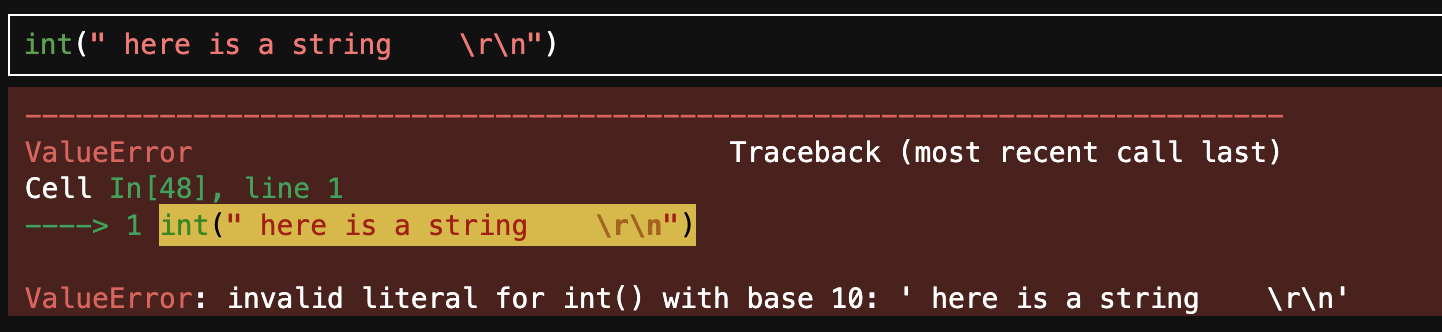
\includegraphics[width=\linewidth]{graphics/python_images/image01.png}
    \caption{A \texttt{ValueError} raised by attempting to convert a \texttt{str}-type to an \texttt{int} type.}
    \label{fig:python-exception01}
\end{figure}

Tracebacks can sometimes be difficult to interpret depending on just how many things went wrong, but the general format is still the same: we are given the name of the exception, the line where this exception occurred, and a statement telling us more information about what went wrong. In this case, we see ``invalid literal for \verb|int()| with base 10:'' and the offending string we tried to convert. 

If we are unsure what type of errors we might get, a safe practice is to use the following syntax:

\begin{lstlisting}[language=Python, showstringspaces=false,backgroundcolor=\color{lightgray}]
try:
    # some statement here
except Exception as e:
    print(e)
\end{lstlisting}

\noindent where we capture the name of the exception in a variable \verb|e| and print it so we know what went wrong. In this situation, as soon as the code encounters an exception it stops executing completely. For this reason, some programmers have taken to using a \verb|pass| statement to skip the offending line code and continue with the rest of the program; as you will see in our workshop sessions, this is \textit{bad Python practice} and can lead to potentially severe problems.

% Now, we present the above with a very important caveat: it is ultimately \textit{bad Python practice!} To see why this can be problematic, examine the following code:

% \begin{lstlisting}[language=Python, showstringspaces=false,backgroundcolor=\color{lightgray}]
% fruits = ['apple', 'pear', 'carrot', 'banana']
% fruit_found = False

% try:
%      for i in range(len(fruit)):
%          if fruits[i] == 'apple':
%              found = true
% except Exception:
%       pass

% if fruit_found:
%     print("An apple is in the list")
% else:
%     print("No apples are in the list")
% \end{lstlisting}

% Before you run this code, try to spot the three mistakes. When you do run the code, you will see the output ``No apples are in the list'', which is clearly incorrect. Why do we get this output? If we adjust our \verb|except Exception:| statement to capture and print the exception, what happens? 

% The big problem here is that our exception catcher tries to catch \textit{all} exceptions, and even if we print those exceptions we have given our code no way to actually fix the problem. This is lazy code, and further violates the Zen of Python (``Errors should never pass silently''). At the very least we want to log the error; but ideally we should attempt to write better code and anticipate the exceptions that might arise. We should only ever use \verb|pass| in these situations as a placeholder to which we can return later and write better code. Remember that the purpose of an exception is to stop our code when something breaks, and if something breaks we probably should try to fix it so it does not break again.

\newthought{Functions \& Modules}

You are aware of functions in mathematics, so we will spare the boring details here. Functions in the programming sense are similar, but are perhaps better thought of as procedures or subroutines within a program. In Python we can define functions with the following syntax:

\begin{lstlisting}[language=Python, showstringspaces=false,backgroundcolor=\color{lightgray}]
def my_function(x):
    y = x*6 + 3
    return y
\end{lstlisting}

\noindent where we pass arguments to the function, the function operates on those arguments, and the function will \textbf{return} a value based on our defined operations. We can call this function simply with \verb|my_function(5)| and get a value. This is similar to our normal understanding of functions and the above code is equivalent to $f(x) = 6x + 3$. 

We can also define our functions to take multiple arguments. We typically talk about \textit{positional arguments} and \textit{keyword arguments} in this scope. Positional arguments are simply assigned in the order they appear; for example 

\begin{lstlisting}[language=Python, showstringspaces=false, backgroundcolor=\color{lightgray}]
    def my_func(x, y):
    ...
\end{lstlisting}
\noindent would work such that the first value you send to \verb|my_func()| when you call it is \verb|x| and the second value is \verb|y|. For functions of few arguments this is fairly simple, but if we have many arguments we may want to use \textit{keywords} instead.

\begin{lstlisting}[language=Python, showstringspaces=false,backgroundcolor=\color{lightgray}]
def my_function(x, a=1, b=2, c=3):
    y = a * x**2 + b * x + c
    return y
\end{lstlisting}

By default this has assigned values to 3 local variables, \verb|a|, \verb|b|, and \verb|c|, so all it strictly requires is the positional argument \verb|x|. These keyword arguments can be overridden, e.g. \verb|my_function(5, a=3, b=2, c=1)|, so that we can exert more control in that way. You have actually already seen this behavior with \verb|open()| in the section on file reading: you provide a filename as the positional argument, and by default \verb|open()| assigns the keyword argument \verb|mode='r'|, which we can choose to override. When using both positional and keyword arguments, the positional arguments must come first.

Using functions helps to ensure our code is \textbf{modular} (the programming motto here is ``Don't repeat yourself''), and allows us to maintain clarity. Our code becomes easier to maintain and provides a well-defined scope for all of our operations. The modular nature is especially important: I can define a function in one file and call it from another file! In fact, this is pretty much what we do when we import Python packages.

At the very beginning we had you use \verb|conda| to install four Python packages. If we are using an IDE or Jupyter, we can import those packages into our workspace quite simply using any of these four methods:

\begin{lstlisting}[language=Python, showstringspaces=false,backgroundcolor=\color{lightgray}]
import module_name
from module_name import some_name
from module_name import some_name as name
import module_name as name
\end{lstlisting}

Any of these approaches is just fine and which one you use depends on what you plan to do. Most people will simply use the shorthand approach, especially for \verb|numpy|, because it is used so extensively that it simply saves time to import it as \verb|np|. 

All Python packages (sometimes called modules) are like libraries of modular code that can be used after importing them as above. These modules can contain variables, functions, and classes that ultimately make our lives easier. In our Jupyter notebooks we will be using in the workshop, you will have plenty of opportunity to explore the functionality of various Python packages. 

\newthought{Plotting \& Visualization}

How can we visualize data in Python? The most widely-used package for this is the \verb|matplotlib| package, and the easiest way to work with it is:

\begin{lstlisting}[language=Python, backgroundcolor=\color{lightgray}]
import matplotlib.pyplot as plt

plt.plot(x, y)
plt.show()
\end{lstlisting}

We can add other arguments to \verb|plt.plot()|, allowing us to adjust the line color, line width, line style, data labels, and so on. We can also fine-tune our control over the figure size and axes using \verb|subplots()|:

\begin{lstlisting}[language=Python, backgroundcolor=\color{lightgray}]
fig, ax = plt.subplots(figsize=(w, h))
ax.plot(x, y)
plt.show()
\end{lstlisting}

We can have a plot with multiple axes too, using the \verb|nrows| and \verb|ncols| keyword arguments. To create a 4-panel plot with 2 rows and 2 columns:

\begin{lstlisting}[language=Python, backgroundcolor=\color{lightgray}]
fig, axes = plt.subplots(nrows=2, ncols=2, 
    figsize=(w, h))
ax[0, 0].plot(x, y)
ax[0, 1].plot(...)
plt.show()
\end{lstlisting}
\noindent where the \verb|axes| object is treated like a nested list.

\newthought{Curve-Fitting}

One of the most important tools for us as physicists and engineers is knowing how to fit a model to data. Assuming we have examined our data closely and decided upon what type of model could best describe it, we can tell Python to do the heavy lifting using \verb|numpy| and \verb|scipy|. 

In short, let us say we have a function $f(x, \theta)$ where $\theta$ represents the parameters of the function. If this is a line, then $\theta = [a, b]$ and this satisfies the function $f(x; a, b) = ax + b$. We want to use $f(x, \theta)$ to model our observable data, and we can do this using a \textbf{least-squares} algorithm. This essentially makes a guess as to the parameters $\theta$ of the function which best fit the data, compares this fitted function to our data and computes the \textbf{residuals}, and continues this process until the difference between the fitted function and the data is minimized. 

If we call our observed value $y_i$, then the residual can be written

\begin{equation}
    r_i = y_i - f(x_i, \theta)
\end{equation}

And the least-squares approach sums up all the squares of these residuals:

\begin{equation}
    S(\theta) = \sum_{i=1}^n \big(y_i - f(x_i, \theta)\big)^2
\end{equation}

The optimized parameters are the parameters which result in the smallest $S(\theta) value$, and we typically do not want to do this by hand. We can, however, define both of these equations as Python functions and use the \verb|scipy.optimize| module to minimize the residuals. The basic syntax is:

\begin{lstlisting}[language=Python, showstringspaces=false,backgroundcolor=\color{lightgray}, breaklines=true]
import scipy.optmize as spo

def my_line(x, a, b):
    return a*x + b

def residuals(parameters, x, y):
    model = my_line(x, *parameters)
    residuals = np.sum((y - model)**2)
    return residuals

best_fit = spo.minimize(residuals, initial_parameters, args=(x, y))
\end{lstlisting}

While this is the basis of countless fitting routines, as it stands this will not give us any information about the errors on our fit, and when dealing with physical measurements we are especially interested in such errors or uncertainties. A better approach is to use the \verb|curve_fit| function, also in the \verb|scipy.optimize| module.

\begin{lstlisting}[language=Python, showstringspaces=false,backgroundcolor=\color{lightgray}]
from scipy.optimize import curve_fit
par_opt, par_cov = curve_fit(my_line, x, y)

\end{lstlisting}

This returns the optimized parameters and the \textbf{covariance matrix} associated with those parameters, and by computing the square root of the diagonals of this matrix we can extract our uncertainties:

\begin{lstlisting}[language=Python, showstringspaces=false,backgroundcolor=\color{lightgray}]
uncertainties = np.sqrt(np.diag(par_cov))
\end{lstlisting}

There are other parameters which can be passed to \verb|curve_fit|, such as boundary conditions and initial guesses, and you are strongly advised to explore the documentation in this regard to gain a better understanding of such usage. Appropriately defined functions are the key to success in this regard, and this might require careful consideration when handling your routines!
\clearpage
\subsection{Exercises}

\textbf{N.B.} These exercises can all be found in the ``Python-workshop-exercises'' notebook on GitHub. The repo additionally contains the data and image files you will need for Tasks 3 and 4.
\begin{tcolorbox}[sharp corners=all, colback=white!75!green]
%[width=\linewidth, sharp corners=all, colback=white!95!black]
\begin{enumerate}   
    \item 
        Print the numbers from 1 to 100 (inclusive), replacing numbers that are divisible by 3 with the string ``Fizz'' and numbers that are divisible by 5 with ``Buzz''. If a number is divisible by both 3 and 5, replace that number with ``FizzBuzz''. 
    % \item 
    %     Alter your FizzBuzz code so that it also checks if the first digit in the number is divisible by 3 or 5 follows the same replacement rules as above. That is, if the number is 52, the first digit 5 is divisible by 5 so you would replace 52 with ``Buzz.''. 
    \item 
        Write a code that generates an integer between 1 and 20, and randomly chooses to either square or cube that number. Store this result, and keep track of which result is the smallest and which result is the largest. If the current number is divisible by the previous number, issue a print statement and exit the loop. After the loop has exited, print the smallest and largest of the squared or cubed numbers, state which two numbers caused the loop to break, and inform the user how many loops the program completed.
    \item 
        Given an optical spectrum from an astronomical source, write a Python script that parses the data file and produces three plots. Your first plot should simply be the full spectrum. Your second plot should contain full spectrum with a polynomial fit to the baseline of the spectrum overlaid. Your third plot should contain the full spectrum, polynomial fit, and a Gaussian fit to the emission peak. Include appropriate axis labels and units, and ensure all elements of the plots are clearly legible. Your script should print the fitted parameters with their uncertainties to the terminal. As a guideline, structure your script so that it can be called simply with
    \begin{lstlisting}[language=Bash]
    $ python my_script.py filename
    \end{lstlisting}
    \item 
        Using the ascent data provided for the Apollo 10 launch, write a python script that parses the file and stores the data from the table columns as arrays within a dictionary, and use this dictionary to make plots of the data. You should plot all 11 parameters as functions of time, and make a plot of the Apollo 10 rocket's ground track. More information about this task is provided in the ``Exercises'' notebook.
\end{enumerate}

\end{tcolorbox} 


\newthought{Recommended Reading:}
\begin{itemize}
    \item \href{https://jakevdp.github.io/WhirlwindTourOfPython/}{A Whirlwind Tour of Python} by Jake VanderPlas
    \item \href{https://greenteapress.com/wp/think-python-2e/}{Think Python (2e)}, by Allen B. Downey
    \item \href{https://python-guide.readthedocs.io/en/latest/}{The Hitchhiker's Guide to Python}
    \item \href{https://lectures.scientific-python.org/}{Scientific Python Lectures}, by dozens of authors and contributors
\end{itemize}

\section{GitHub}\label{sec:github} %

% \sidenote{Recommended Reading: 
% \begin{itemize}
%     \item Pro Git, by Chacon \& Straub
% \end{itemize}}
{Another} (indispensable) tool we will be using is called \textit{Git}\footnote{\href{https://git-scm.com/}{https://git-scm.com/}}, which is a ``distributed version control system'' that allows you or multiple others to simultaneously work on a similar project while keeping track of different versions of the project. It is far more efficient than simply saving multiple versions of a similar file, and it is vastly superior to standard word processing software which can only keep track of a limited number of recent changes (that is, you can only \texttt{ctrl+z} or \texttt{ctrl+y} so many times in a single document). With Git, you will always have a record of what you've done so you can revert to an older version if need be, and all the different changes you or other people have made can ultimately be merged into a single source, making this particularly useful for programming teams.

% \begin{figure}
%     \centering
%     
\includegraphics[width=0.8\linewidth]{graphics/github/phd101212s.png}
%     \caption{Revision is a common issue when writing any sort of documentation. Image from \href{https://phdcomics.com}{PhD Comics}.}
%     \label{fig:final-notfinal}
% \end{figure}

There are many platforms on which to use the Git architecture, most notably {\href{https://www.github.com}{GitHub}} and {\href{https://www.gitlab.com}{GitLab}}, and on both of these online platforms you can find just about any open-source project or software you can imagine. For this course we will be using GitHub, so you need to navigate to their site and set up your own account using your school email. Details on the installation and setup of \verb|git| on your local machine will be discussed below.
%If you have little or no experience using the command line, you can use the {\href{https://docs.github.com/en/desktop/overview/getting-started-with-github-desktop}{GitHub Desktop}} Graphical User Interface (GUI), which is available for Mac and Windows.\footnote{If you are using the command line on Mac or Linux, then you know what you're doing so you don't need any help here.} This is recommended over trying to use the browser to manage your workflow as it is simply an easier interface and helps keep things neat and organized. You can follow the link above to install the GUI on your machine.

\subsection{Understanding the GitHub workflow}\label{subsec:git-workflow} %

{There are three} major concepts with which you will want to familiarize yourself when utilizing the git architecture: repositories; cloning; and committing and pushing. We provide a brief summary of each below, and will discuss them further in turn.

\textbf{Repositories} (or \textit{repos} in shorthand) are simply a place to put your work. A repo functions essentially like a folder or directory on your computer, which we call the local machine. On GitHub, these repositories are stored in a cloud which we call a remote. The repository for a project contains all of that project's files and revision history -- everything you've done is kept here. 

\textbf{Cloning}, as the name implies, allows you to make a local copy of a repository (that is, you can save it to your computer). When you clone a repository GitHub pulls down \textit{all} of the data from that project to your machine, giving you access to every version of every file and folder of the project. When you alter the local copy on your computer, you can use Git to sync your local copy to the remote copy. This makes it easy to edit code or fix issues, and also to add or remove entire files or folders that you may not need for your project. %Cloning is done either through the command line interface (this author's preference) or through the GitHub Desktop application. 

\textbf{Committing and pushing} are the collective process by which you take all your edits and changes for a project and add them to the remote repository. When tell Git that you want to \textit{commit} certain files, it keeps track of them in your repository and makes a ``checkpoint``. It is best practice to include useful \textit{commit messages} so that other contributors can have an idea of what changes you made. Once you've committed all your files and folders that you want to be part of your project, you use the \textit{push} command to tell Git to add those changes to the remote repository. 
% Why github is important, what is is, some basics of how to interact with it

\newthought{In each repository} we begin with a default ``branch`` (or version of that repository) which we call \verb|main|. By longstanding tradition, programmers are expected to reserve the \verb|main| branch for the final, publishable version of their project or code. If we want to make a change or add something to our project but we do not want to change the primary code, we create a different branch with a descriptive name and make any edits on the code there. If we are working as part of a group, we can create something called a ``pull request`` that lets the other collaborators know we have proposed a change to the code, and (if all goes well) merge our branch with \verb|main|, as seen in Figure~\ref{fig:git-branch-flow}. 

\begin{figure*}[h]
    % \centering
    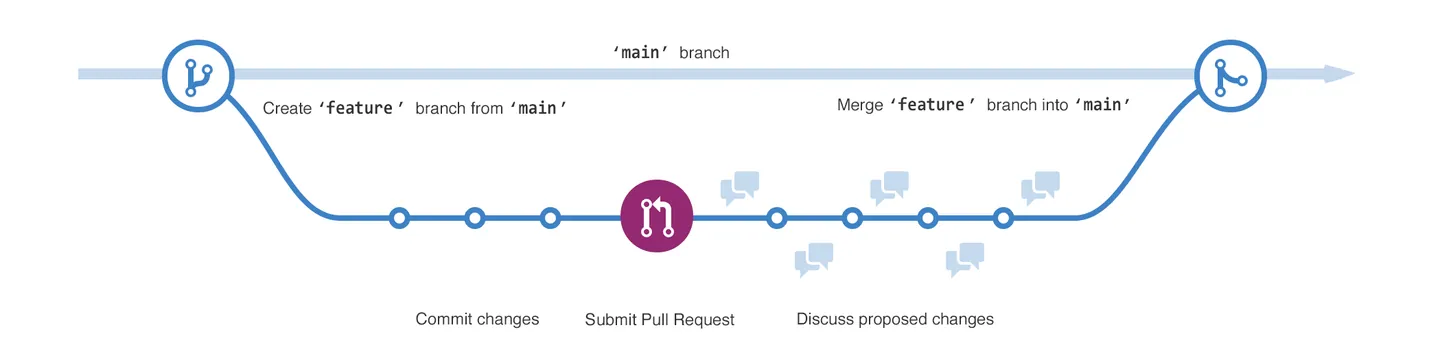
\includegraphics[width=0.9\linewidth]{github/branching}
    \caption{A schematic demonstrating the ``branching`` of a repository; from GitHub.com.}
    \label{fig:git-branch-flow}
\end{figure*}

The branching process can be as simple or as complicated as we like. For example, we could create a branch of \verb|main| called \verb|development| where we do the majority of our work. We merge our \verb|development| branch occasionally with \verb|main| to create different official versions of our program, e.g. V2.0 or V2.1. Something in \verb|development| breaks, so we create a branch called \verb|hotfix| to try to fix the issue. However, during the process we break something else, so we create another branch called \verb|hotfix-hotfix| to address that issue. These two hotfixes get merged into our \verb|development| branch. While working on that, we also decide we want to add a new feature to our code so we create a branch called \verb|feature| to handle this. A rudimentary flowchart of such a workflow is shown in Figure~\ref{fig:complex-workflow}. 

\begin{figure*}[h]
    % \centering
    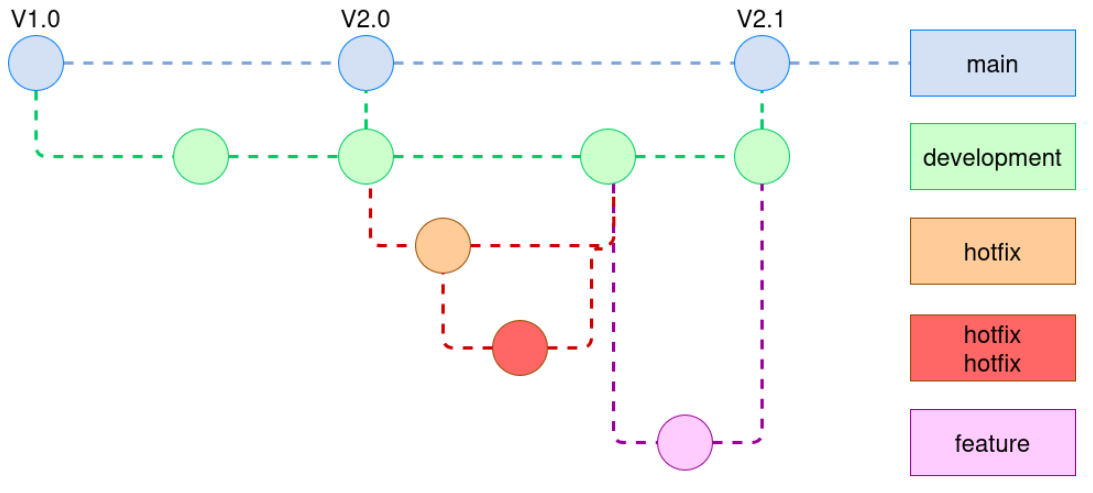
\includegraphics[width=\linewidth]{graphics/github/github-branch-flow}
    \caption{A fairly typical workflow for a software project.}
    \label{fig:complex-workflow}
\end{figure*}

With larger projects this can become even more complex, where we might have different \verb|feature|-type branches for different software editions we make, and multiple people might have their own \verb|hotfix| branches or even separate branches representing their own team's work. No matter the scenario, the process is the same: we pull the latest version of the project and its branches, we move to some branch we want to work on, we commit and push our work to that branch, and eventually merge all the working code into the primary branch.

\subsection{Installation \& Configuration}\label{subsec:git-install} %

To use Git we need to have it installed on our local machine, and it needs to be configured. For this module and other modules in this course, you will maintain your code on an organized repository and submit the repository link to us. As mentioned above, you need to sign up for a GitHub account using your school email (not a personal email). Assignments will be provided to you through BrightSpace as ``GitHub Classroom'' instances, and when you accept an assignment you will be added to the Classroom and we will have an easy way to see your progress.

\newthought{The preferred method} of installation for this course is through the \verb|conda| environment, though you may choose to use the {\href{https://docs.github.com/en/desktop/overview/getting-started-with-github-desktop}{GitHub Desktop}} Graphical User Interface (GUI), which is available for Mac and Windows.\footnote{If you are using the command line on Mac or Linux, then you know what you're doing so you don't need any help here.} Once it is installed you will need to configure the Git software with your name and email before you can make any commits to your repo. This is done through the command line:

\begin{figure*}
\begin{lstlisting}[backgroundcolor=\color{lightgray}]
$ git config --global user.name "Firstname Lastname"
$ git config --global user.email "YourStudentEmail"
\end{lstlisting}
\end{figure*}

Note that using your email here can pose a security risk. To mitigate this risk, you are encouraged to use the GitHub \verb|noreply| email address that GitHub provides to users. Go to \texttt{github.com} and navigate into your account settings, where you can select ``Keep my email address private'' in the Email settings options. More about this can be read on the \href{https://docs.github.com/en/account-and-profile/setting-up-and-managing-your-personal-account-on-github/managing-email-preferences/setting-your-commit-email-address}{GitHub docs} page ``Setting your commit email address''.

Next you need to configure a \textbf{personal access token}. You can follow the steps on the GitHub documentation to do this. If you do not wish to re-enter your credentials every time you make a push or a commit, you can tell Git to store your credentials on your local machine:

\begin{figure*}
\begin{lstlisting}[backgroundcolor=\color{lightgray}]
$ git config --global credential.helper store
\end{lstlisting}
\end{figure*}

\subsection{Basic Operations}\label{subsec:basic-ops} %

Above we discussed some concepts that are fundamental to the git workflow. When working with Git, there are some essential command-line operations that you should devote to memory. 

\begin{itemize}
    \item \verb|git add| --  add a new file to the repository
    \item \verb|git rm| -- remove a file from the repository
    \item \verb|git mv| -- rename a file in the repository
    \item \verb|git fetch| -- check the remote repository for changes
    \item \verb|git pull| -- pull the most recent changes from the remote repository into your local repository
    \item \verb|git push| -- push local changes to the remote repository
    \item \verb|git commit| -- save your changes as a new version in the repository
\end{itemize}

This is not an exhaustive list, and you are encouraged (expected, even) to consult the additional materials on the module BrightSpace page.

So, what do we do with all of these, and how to we interact with GitHub? If you followed the tutorial documentation on the GitHub site (which you should definitely do) then you will have noticed that on every GitHub repo webpage there is an option to clone the code, as in Figure~\ref{fig:git-clone}. The two most common options are to clone a repo over HTTPS or over the \textit{secure shell protocol} (ssh), but you can also use the GitHub CLI, GitHub Desktop, or even download a ZIP archive if you want. For one-off software downloads the ZIP archive is okay, but if you are consistently pulling from and pushing to a repo you should really use the \verb|git clone| method.

\begin{marginfigure}
    \centering
    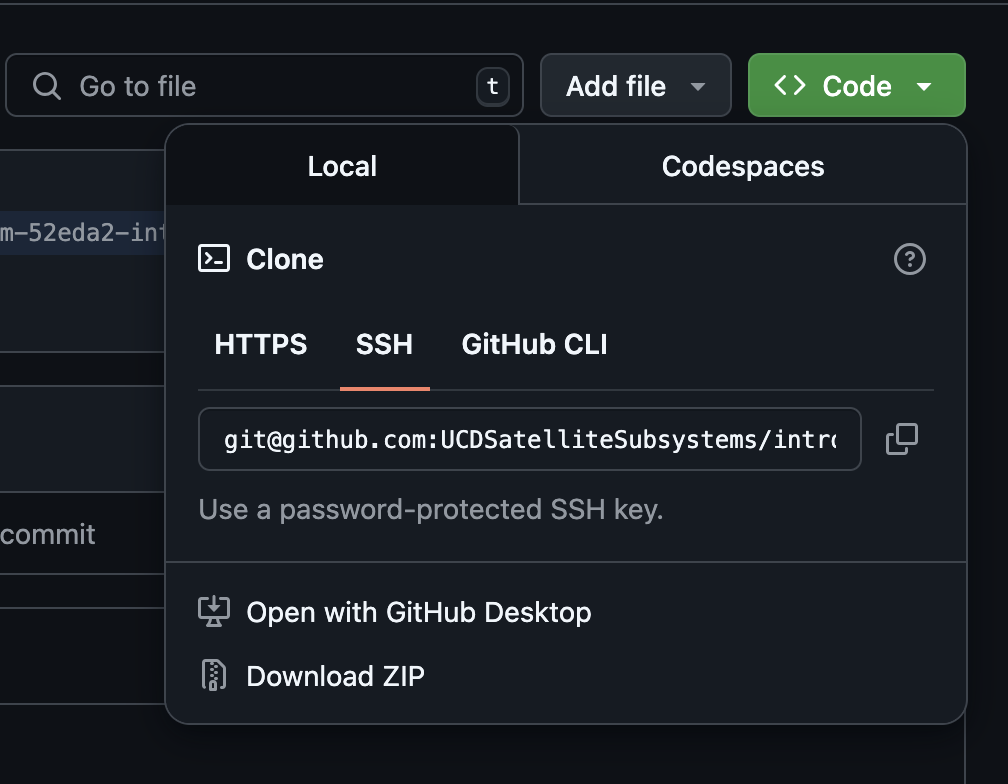
\includegraphics[width=\linewidth]{graphics/github/git-clone.png}
    \caption{The \texttt{clone} options available on the browser interface of a GitHub repo.}
    \label{fig:git-clone}
\end{marginfigure}

With HTTPS, you will be prompted for a username and password unless you have stored your credentials. When using the UCD Wireless network, we have found that sometimes HTTPS is more reliable due to the UCD firewall. If using ssh, you will need to set up a ``public key'' that your local machine will use to authenticate all of your transactions.\footnote{see \href{https://docs.github.com/en/authentication/connecting-to-github-with-ssh/about-ssh}{Connecting to GitHub with SSH} in the GitHub documentation.}

Now, you simply open a terminal and type in your commands. If we want to clone the \href{https://github.com/skills/introduction-to-github}{Introduction to GitHub} repo using the HTTPS protocol, then we can type:
% \begin{itemize}
% \end{itemize}

\begin{figure*}
\begin{lstlisting}[backgroundcolor=\color{lightgray}]
$ git clone https://github.com/skills/introduction-to-github
\end{lstlisting}
\end{figure*}

All going well, you should have successfully cloned into the \verb|introduction-to-github| repo. This will automatically create a new folder in whatever working directory we are using -- for example, if I was in my ``My Documents'' folder then I will see a new folder where the repo was cloned. Whenever I use my Git commands, I want to be in that newly created folder. 

There is a very important thing to point out here, however. This just creates a local repo that points to the original URL I cloned, and if I try to push or commit any changes I might find it difficult because I am not the owner of that GitHub repo nor have I been given any permissions for contributing. So, how can I make changes and commit them to a repo under my own username? To do this I need to \textit{fork} the repository -- this creates a copy under my own username -- and then clone the fork. For the majority of our classwork you will not have to worry about this: when you accept the GitHub Classroom assignments, it automatically forks the repository under your own username. 

Try it yourself: go to the \verb|introduction-to-github| repo, create a fork under your username, clone the fork. In that directory, create a new text file with ``Hello, world!'' in the body and commit and push it to your repo. Did it work?

%\begin{fullwidth}
% \begin{lstlisting}[backgroundcolor = \color{lightgray},caption=Example code,label=fig:header]
% Here is some example code of how to interact with github
% \end{lstlisting}
%\end{fullwidth}

% \section{Virtual environments}


% \begin{lstlisting}[backgroundcolor = \color{lightgray},caption=Example code,label=fig:header]
% Here is some example code of how to set up conda
% \end{lstlisting}

\newthought{Recommended Reading:}

\begin{itemize}
    \item \href{https://git-scm.com/book/en/v2}{Pro Git}, by Chacon \& Straub
    \item \href{https://docs.github.com/en/get-started/start-your-journey/git-and-github-learning-resources}{Using GitHub}, on the GitHub documentation page
\end{itemize}

\section{Using LLMs for coding}

Since the first release of ChatGPT in 2022, Large Language Models (LLMs) have been rapidly adopted across many areas of society. It is clear that LLMs will continue to improve in capabilities over the years to come, and that they are set to feature in all areas of society (including science) in the future. With this in mind, we do not wish to make a blanket ban on AI, but rather invite students to consider their use of this, and to ensure that if they use LLMs or other tools, they do so responsibly.

LLMs have proven extremely good at writing code. In fact, if you ask an LLM to write some Python code to solve a textbook coding problem (for example, writing an implementation of bubble sort), it will likely do so correctly. This performance most likely reflects the structured nature of coding languages, as well as the vast amount of example code on which LLMs have been trained. Where LLMs will perform less well is on problems that are more niche, or where there are multiple steps involved. The danger is that an AI may produce some code that perhaps works, but misses critical steps or incorrectly implements an algorithm that an inexperienced user may miss\footnote{This is an excellent example of the proverbial ``chimp with a machine gun''}. In these cases, what is necessary is to break the problem down into small chunks that the LLM {\it can} handle.

As an example let us ask ChatGPT to write some code to do point spread function (PSF)-fitting photometry on some HST/ACS images (don't worry if you don't know what this is -- it's a fairly standard type of data analysis that one would run on Hubble Space Telescope images). If we prompt ChatGPT as follows

\begin{lstlisting}[backgroundcolor=\color{lightgray}, breaklines=true]
I would like some code to do PSF-fitting photometry on HST ACS images. Images will need to be aligned, a PSF model built and photometry calibrated onto a standard system
\end{lstlisting}

\noindent then what we get back is code that will run, but give completely incorrect results. More specifically, the prompt to "align the images" results in code that assumes the World Coordinate System information in each image is correct, while in reality there will be $\sim$few pixels offsets that must be accounted for. Similarly, the code builds a model of the PSF from {\it all} sources in the field, whereas best practice is to use bright, isolated stars to model the PSF. Again, the key point is that you get something that is superficially correct and will run, but that has serious and fundamental errors.

To avoid this, if one is using LLMs to write code then it necessary to break the problem down into sections. The overall structure of the solution is generally something that the user can (and should) design. In this case, before beginning we might decide that our code needs to align pairs of images, build a PSF, detect sources, fit a PSF to each source, and calibrate the resulting value. Here, one could prompt ChatGPT with more granular instructions, and iterate to build code rather than doing this in a single step. For example, just to align the images we could use the following prompts

\begin{lstlisting}[backgroundcolor=\color{lightgray},breaklines=true]
I would like to write some python code using the astropy library to read in a fits file.
\end{lstlisting}

then

\begin{lstlisting}[backgroundcolor=\color{lightgray}, breaklines=true]
I would like to calculate the pixel offset in x and y from a second fits image by doing a two-d cross-correlation with scipy.
\end{lstlisting}

then 

\begin{lstlisting}[backgroundcolor=\color{lightgray}, breaklines=true]
Finally, I wish to measuring the position of the cross-correlation peak by fitting a 2d Gaussian to it.
\end{lstlisting}

As you can see, we are building our code in a much more iterative fashion. We are giving explicit instructions on how we want ChatGPT to solve the problem, and we are also doing it in a way that we can look at the output at each step to see if it as expected, rather than simply 
seeing the final result\footnote{\raggedright{This has been described as \href{arstechnica.com/ai/2025/03/is-vibe-coding-with-ai-gnarly-or-reckless-maybe-some-of-both/}{vibe coding}.}}.

Even doing this, LLMs can still make mistakes. So, it is critical to build tests and ``sanity checks'' into your code to help ensure that the output is correct. Taking the example above, one could easily plot the two images, and the shift, and visually confirm that they are aligned. Also, keep in mind that even if the code that is produced by an LLM works, it may not be particularly ``good'' code, or an optimal or efficient solution.

It is also important to remember that while LLMs have been trained on a vast corpus of code, the more obscure and niche the problem, the less useful they will be. Usually, your specialist expertise will still be needed to write the core of whatever code is needed: designing an algorithm to model the temperature increase when a thruster fires, or inferring rotation rate from solar panel data on a tumbling satellite. Remember that this is where your value and skill-set lies, and that while it will often be fine to use LLMs for much of the boilerplate code surrounding a problem (for example, reading and parsing some datafiles into a \verb|numpy| array), the core of what you are trying to do will usually require human expertise and experience. 

The guidance above pertains to using LLMs to write code. The advice for writing text is quite different. It is important to keep in mind that LLMs work by forming associations between tokens and patterns. As they do not have any understanding of what they are producing, it is inherently risky to use them to write introductions, or indeed any other parts of a report or document. While code produced by an LLM can be tested, and we can satisfy that its outputs are correct, we cannot do such a test for, say, a description of how a Hall thruster works.

Aside from the major problem with using LLMs for writing, namely that it has no {\it understanding} of what it outputs\footnote{See \href{https://link.springer.com/article/10.1007/s10676-024-09775-5}{this article} for an entertaining discussion on this point.}, there are other more subtle downsides:

\begin{itemize}
    \item  Over the course of your MSc, we want you to acquire a broad range of skills relevant to the space sector. One of the best ways of learning information and reinforcing it is by explaining to others, whether in the form of an oral presentation or writing a report or essay. Using LLMs to summarize a topic negates this - even if you feel you know what you are writing about, you are more likely to retain this information into the future by writing it down yourself.
    \item It is also easy to develop a habit of turning automatically to LLMs, even when they are not the best tool to use in that moment - for example, if there is a human expert readily available.
    \item Some LLMs will often structure output in condensed snippets or bullet points that, when used in academic or scientific writings, can severely undercut the importance of the point the author is trying to convey.
    \item Most industry and government bodies have very strict rules around data confidentiality and security. Using an LLM from a third party can result in loss of proprietary information. 
\end{itemize}

As a final note, we may also be concerned about the the environmental impact that systems support LLMs can have For example, a single Google search uses about 10\% of the Wh required to ask ChatGPT the same thing.\footnote{See \href{https://www.rwdigital.ca/blog/how-much-energy-do-google-search-and-chatgpt-use/}{here} for reference, as well as \href{https://www.rwdigital.ca/blog/how-much-energy-do-google-search-and-chatgpt-use/}{the MIT Technology Review} series on the subject.} While this may amount to comparatively very little for a single user, as the number of users of LLMs grows the energy usage increases significantly; according to the CSO\footnote{\href{https://www.cso.ie/en/releasesandpublications/ep/p-dcmec/datacentresmeteredelectricityconsumption2024/}{CSO Statistical Release}, ISSN 2811-5422}as of 2024, data centers in Ireland accounted for nearly a quarter of all electricity usage in the country -- an increase of over 500\% since 2015. While of course the overall impact of LLMs and data centers is far beyond the scope of this course, as scientists we should nevertheless seek to understand the tools we use so that we can make informed decisions about our relationship with those tools.\footnote{See, if you are interested, \href{https://mit-serc.pubpub.org/pub/the-cloud-is-material/release/2}{The Cloud is Material} for one opinion (of many) on this subject.}

\begin{tcolorbox}[sharp corners=all, colback=white!75!red]
Key points for using LLMs in this module
\begin{itemize}   
\item An LLM is a tool. Always use it consciously, deliberately, and with a clear understanding of what you are doing.
\item Any use an LLM for assistance with coding must be clearly identified and acknowledged.
\item Do not use LLMs for writing or generating text in reports or assignments. If you use an LLM for language editing, then you should identify this, and also submit the (non-edited) version of the report alongside any language-edited text.
\end{itemize}
Note that each module will have its own rules regarding the use of AI, and you should follow these.
\end{tcolorbox} 



% \chapter{High energy detectors}

% \section{Theory and background}

% Types of detector, physics principles


% \section{Experiment}


% \begin{tcolorbox}[sharp corners=all, colback=white!75!green]
% %[width=\linewidth, sharp corners=all, colback=white!95!black]

% What to do for the experiment here

% \begin{itemize}
% \item Code to do calibration curve (channel to wavelength)
% \item Code to get energy resolution (FWHM of photopeaks) and make a plot as a function of energy
% \item Code to get efficiency, absolute, intrinsic plotted as a function of enerhy
% \item Off axis response (change in FWHM and peak height) 
% \end{itemize}

% \end{tcolorbox} 

% \section{Comparing results}

% Get results from github for other groups. Plot a sensitivity curve etc for all four detectors

opti\chapter{Optical and other detectors}


\section{Theory}

\section{HST images}



\section{SENTINEL-2 images}

\chapter{High energy detectors}

\begin{tcolorbox}[colback=red!5,colframe=red!75!black,title=\textbf{Important
      --- Radiation Safety}] 
The radioactive sources in the lab are low intensity sources (provided they remain outside your body) but you must take certain sensible precautions: 
\begin{enumerate}
\item Sources must only be used with the explicit consent of the lab instructor. 
The sources must be signed in and out, and only by the lab instructor. 
\item The sources must be handled carefully. Plastic tweezers should be used
  when handling to protect the sources. Hold them at the top or the edge. Do
  not hold them in the center (either with tweezers or with fingers) --- there
  is a risk that you will damage the protective slide. 
\item There shall be no food or drink in the laboratory. 
\end{enumerate}
\end{tcolorbox} 

Gamma-ray astronomy is the study of astrophysical objects via the detection of their energetic photons, which can range from 10 keV to hundreds of GeV in energy. Energies below 10 keV are generally described as being x-rays.

In order to efficiently detect \textgamma-ray emissions from astrophysical sources, the correct scintillator and/or detector combination needs to be used, as each detector is sensitive over a particular part of the electromagnetic spectrum, with a quantum efficiency that varies with respect to energy.

In this lab you will calibrate and characterize different \textgamma-ray detectors. Each type has flown on past and present \textgamma-ray astronomy missions. You will examine the behavior of these detectors and write a report discussing their performance and suitability for different space missions.

The experiments you do will follow the pre-flight tests performed ont he detectors for the Fermi Burst Alert Telescope, documented in Bissaldi et al. (2009). You should read this paper, which can be found on BrightSpace. 

You will be assessed based on your code, which is to be submitted to GitHub, and your final report, which is to be no less than 5 pages and no more than 10 pages including tables and figures. Your final report should include both a presentation of your results and a discussion about the characterization of the detectors and their suitability for space missions.

\section{Theory and background}

\gmray~ detectors work by converting the energy deposited by high-energy photons when they interact with the detector material into measurable electrical signals. To do this, they use the deposited energy to excite electrons within the crystal structure. These excited electrons generate an electrical signal, which is measured and digitized. Since the number of excited crystal electrons increases with the amount of energy deposited in a detector, the size of this response measures the energy deposited by the \gmray.\footnote{While the energy deposited by each incoming photon is typically tens to hundreds of keV, the bands within the crystral structure of the detector crystal are typically on the order of a few eV. This means that the energy deposited by each high-energy \gmray\, produces a macroscopically detectable number of excitations, and so a measurable detector response.}

For each incoming photon, the output from the detector is digitized. This adds a count into the appropriate digital energy channel. Once many \gmray s have entered the detector and deposited (some or all of) their energy, the resulting spectrum consists of the number of counts in each channel.

The detectors you are required to investigate are:

\begin{itemize}
    \item 
        a Cadmium Telluride detector (CdTe);
    \item  
        a Thallium-doped Sodium Iodide detector (NaI:Tl); and
    \item 
        a Bismuth Germanate detector (BGI).
\end{itemize}

These represent two types of detector, which are distinguished by how they convert excited electrons into an electrical output. These are:

\begin{itemize}
    \item 
        Solid state detectors (CdTe and high-purity germanium, or HPGe) directly detect the energy absorbed from ionizing radiation as an electrical current generated when the high energy photon deposits energy and excites electrons into the conduction band of the material.
    \item 
        Scintillator detectors (NaI and BGO) have crystals which absorb high-energy photons and re-emit low-energy photons at visible wavelengths. A photomultiplier (usually a photomultiplier tube [PMT]) is used to convert this light into an electrical signal that can be amplified and digitized.
\end{itemize}

Make sure that you understand the differences between the physics of these two detector types: they are fundamental to understanding the similarities and differences between the resulting spectra. You will need to address this topic in your report and use it to inform you discussion.

\subsection{Radioactive sources}

You will use pre-calibrated radioactive sources to determine the spectral response of the lab detectors. We will use 4 radioisotopes in this lab. These radioisotopes consist of unstable nuclei, which decay over time via \textalpha, \textbeta, or \textgamma-decay to a stable nucleus. The decay schemes for these radioisotopes are shown in Table~\ref{tab:source-activities}.

\begin{table*}[h]
% \begin{fullwidth}
  \centering
  \begin{tabular*}{\textwidth}{@{\extracolsep{\fill}}c c c c c}
    \toprule
    Isotope
    & Decay Mode
    & Half-life $\tau_{1/2}$ / yr
    & Energy / keV
    & Emission Fraction \\
    \midrule
    $^{60}$Co  & \betaminus  & $5.2714(5)$ & $1173.228(3)$  & $0.9985(3)$   \\
               &             &             & $1332.492(4)$  & $0.999826(6)$ \\
    \addlinespace[6pt]                                      
    $^{133}$Ba & EC          & $10.537(3)$ & $53.1622(6)$   & $0.0214(3)$   \\
               &             &             & $79.6142(12)$  & $0.0265(5)$   \\
               &             &             & $80.9979(11)$  & $0.329(3)$    \\
               &             &             & $276.3989(12)$ & $0.0716(5)$   \\
               &             &             & $302.8508(5)$  & $0.1834(13)$  \\
               &             &             & $356.0129(7)$  & $0.6205(19)$  \\
               &             &             & $383.8485(12)$ & $0.0894(6)$   \\
    \addlinespace[6pt]       
    $^{137}$Cs & \textalpha  & $30.09(11)$ & $661.657(3)$   & $0.8499(20)$  \\
    \addlinespace[6pt]       
    $^{241}$Am & \textalpha & $432.2(6)$  & $26.3446(2)$   & $0.024(3)$    \\
               &             &             & $33.1963(3)$   & $0.00121(3)$  \\
               &             &             & $59.5409(1)$   & $0.3578(9)$   \\
    \bottomrule
  \end{tabular*}
  \caption{Properties of nuclides used in this experiment, including decay
    modes, half-lives, and photon energies of major emission peaks. Data from
    appendix B of Gilmore et al. 2008} \label{tab:source-activities}
    % \end{fullwidth}
\end{table*}

For decay by \textalpha\, emission, we may look at $^{241}$Am as an example to help us understand the process. This has a half-life of 432 years, and decays to $^{237}$Np by emitting an alpha particle, which is just $^4_2$He. In doing so, it populates excited levels in $^{237}$Np, one of which is the $^{5^-}_2$ level at an excitation energy of 59.5 keV. After 67 ns, this level decays to the ground state of $^{237}$Np via emission of a 59.5 keV X-ray.

$^{60}$Co  on the other hand has a 5 year half-life and decays by \betaminus\, emission to $^{60}$Ni. This decay populates the $4^+$ excited state in $^{60}$Ni, which promptly undergoes a rapid cascade (on picosecond timescales) to the ground state in this stable nucleus, emitting two \textgamma-rays with energies of 1173.2 keV and 1332.5 keV.

Table~\ref{tab:source-activities} contains some details about the principal emission lines that you will encounter inthe lab, including the nominal energy of the transition and the fraction of decays that result in emission of a photon of that energy. Note, this table does not contain all the emission features seen with these isotopes. You would need to consult catalogs of reference spectra to correctly identify all the decay features, especially when trying to analyze lower-energy features in spectra from high-resolution detectors. One example of such a databse is the \href{https://gammaray.inl.gov/SitePages/catalog_ge.aspx}{Gamma-ray Spectrometry Catalog}, hosted by the Idaho National Laboratory.

\begin{figure*}
    \centering
    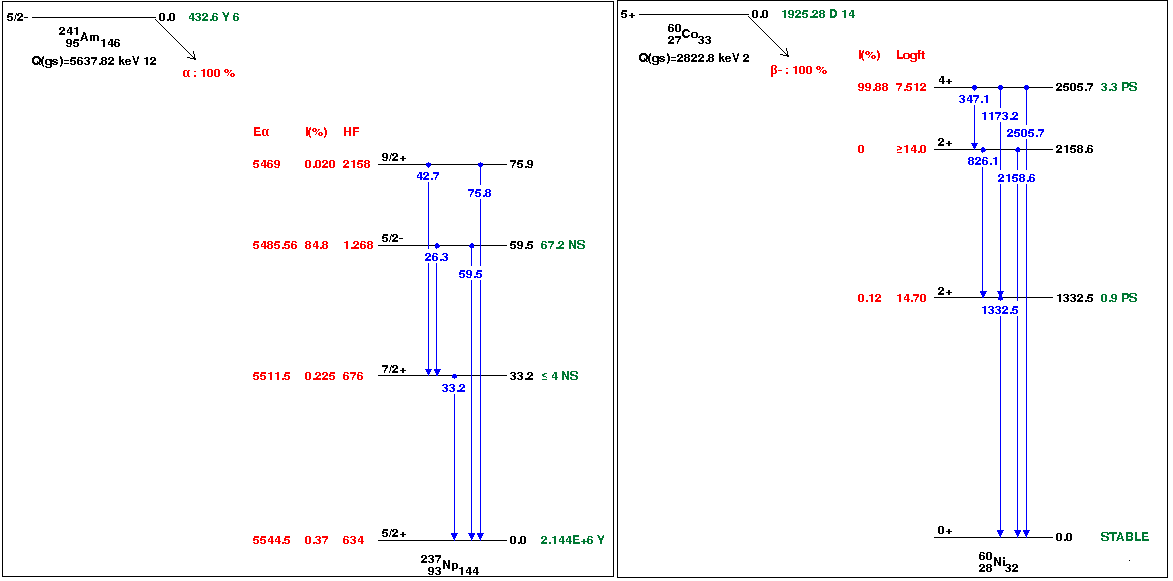
\includegraphics[width=0.9\linewidth]{graphics/he_detectors/decayscheme.png}
    \caption{Left: the decay scheme of $^{241}$Am to $^{237}$Np showing the 60 keV transition. Right: The decay scheme of $^{60}$Co to $^{60}$Ni, showing the prompt cascade of the 1173 and 1332 keV transitions. Images are modified from Brookhaven National Laboratory.}
    \label{fig:decay-scheme}
\end{figure*}


\subsection{Basics of Gamma-Ray Spectra}

The radioactive source emit discrete energy lines. However, the energy spectra produced by the detectors are much more complex. High-energy photons interact with the detector by 3 principal methods:

\begin{enumerate}
    \item the photoelectric effect;
    \item Compton scattering; and
    \item pair production.
\end{enumerate}

These combine to produce complex spectra like that shown in Figure~\ref{fig:cs137-spectra}. The spectrum has been produced by a monochromatic source (that is, a source emitting photons of a single energy; namely 662 keV for $^{137}$Cs). We might expect that this would produce a narrow peak corresponding to that emission line; however, while we can see a clear peak (termed ``photopeak''), there are also features at lower energies caused by photons that have only \textit{partially deposited} their inident energy in the detector. Partial deposition can occur if either the $\gamma$-photon or the products of its interaction escape the detector after its first interaction.

\begin{figure}[h!]
    \centering
    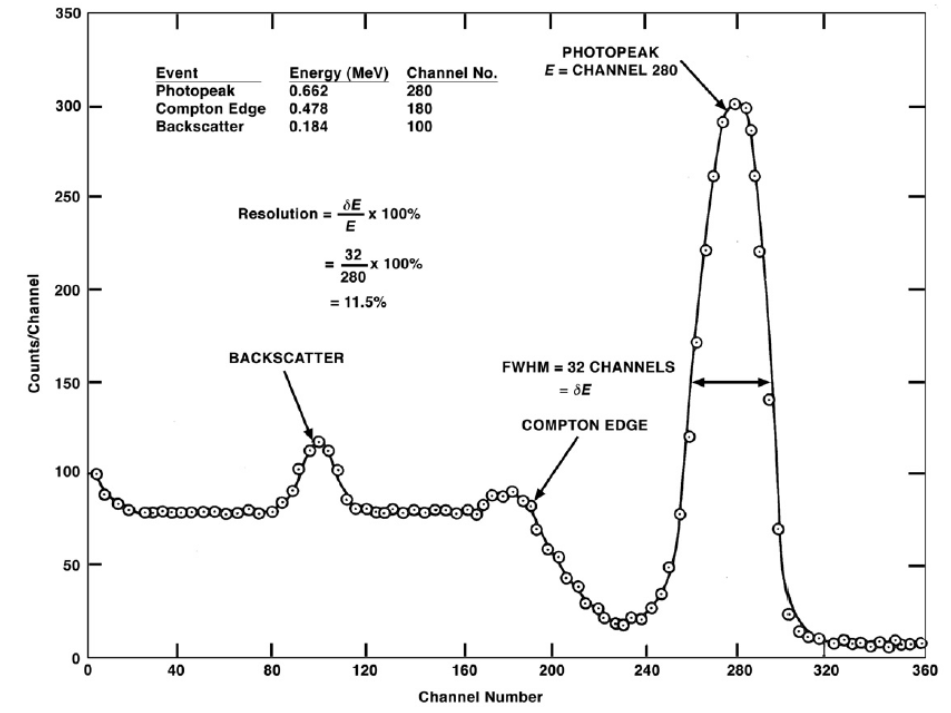
\includegraphics[width=0.8\linewidth]{graphics/he_detectors/137Cs_spectrum.png}
    \caption{An energy spectrum showing the 662 keV photo-peak of $^{137}$Cs as detected by a NaI:Tl detector. Figure originally from Oregon State University.}
    \label{fig:cs137-spectra}
\end{figure}

In this figure, we see the following features:

\begin{itemize}
    \item the Compton feature, a continuous spectral feature caused by \textgamma-rays scattering off electrons and then escaping the detector;
    \item the electron-position escape peaks, where pair production happens close enough to the edge of the detector that one or both of these particles escapes, carrying away its rest-energy; and
    \item X-ray escape peaks, where a \textgamma-ray undergoes photoelectric absorption near the detector surface and the resulting photoelectron escapes, carrying away its kinetic energy and leaving behind just the binding energy taken to eject it.
\end{itemize}

In principle, if the source activity is high compared to the detector response and readout times, we may also see significant numbers of counts above the photopeak due to count pile-up. This happens when two photons enter the detector sufficiently close together in time so that the detector cannot distinguish between them. In practice, unless the source is very active or the detector takes a very long time to process each \textgamma-ray event, pile-up happens so rarely that the spectrum falls off rapidly beyond the photopeak. You will need to discuss these processes in your final report.


\section{Experiment}
\label{sec:he-experiment}

\subsection{Problem statement}
\label{subsec:he-prob-state}
For this portion of the laboratory you will be tasked with calibrating and characterizing the performance of the detectors. This is done so that you can compare and contrast the detectors, commenting on similarities and differences, as well as strengths and weaknesses, and comment as well on the suitability of certain detectors for certain missions. 

Because our spectral data is composed of channels and counts, you must first calibrate each detector to determine its energy response. To characterize the performance of a detector, you must determine: 

\begin{enumerate}
    \item the energy resolution as a function of energy;
    \item the absolute and intrinsic efficiencies as functions of energy; and
    \item the off-axis performance of the detector, e.g. efficiency as a function of angle.
\end{enumerate}

You will need to develop an appropriate set of \textbf{data analysis pipelines}, which means that you will write a set of scripts that take inputs as spectral files and appropriate configuration information, and output the appropriately analyzed data products, including tables and graphs.

\subsection{Data Collection}
\label{subsec:he-data-collect}
You will collect your data from the specified detectors, working in small groups and sharing this data with your team members. It is your responsibility as a group to ensure clear communication among yourselves, such as agreeing on a consistent approach to documenting data collection, naming conventions, and so on. Be aware that if any information is missed, there may not be time to repeat the data collection.

\subsection{Data Extraction \& Analysis}
\label{subsec:he-analysis}
The spectra will be saved as either \verb|.mca| (for the CdTe detector) or \verb|.Spe| files (for NaI and BGO), which are plain ASCII text files. These can be opened with any text editor (such as Notepad on Windows or TextEdit on Mac), which means they can also be read with Python.

Within your pipeline, you will probably need to write Python functions that take the files, return the spectrum (and any important metadata) in a common format to pass to the next stage of the pipeline.\footnote{It would be wise to plan ahead in this regard, and create a clear ``action plan'' for processing your data.}

Once the data is collected, you will need to analyze it by fitting models to the spectra. A best approach is to fit a parametric model to each of the photopeaks, as you can determine the parameters of that model (e.g. line position, width, and area) and use these results in your calibration and characterization.

Typically when dealing with spectra, our first approach is to fit a Gaussian line profile of the form:

\begin{equation}
    f\left(x; \mu, \sigma^2, A\right) = \frac{A}{\sigma \sqrt{2\pi}}\exp \left(-\frac{(x - \mu)^2}{2\sigma^2}\right)
\end{equation}

\noindent While this is a good place to start, it is not going to completely describe both the continuum and the line; and in some cases, particularly where there are multiple poorly resolved decay channels, it may not be possible to fit the spectral line components separately.

As such your pipeline should be able to handle compound models that are more complex than a simple Gaussian. You may choose to fit a Gaussian superimposed on a low-order polynomial as a first attempt. This would allow you to extract your Gaussian parameters as well as the ``nuisance'' background parameters which you can likely ignore.

It is also advisable to attempt to fit one line at a time. It may be tempting to fit the whole spectrum, but the actual shape is incredibly complicated and requires considerable physical modeling, which is beyond the scope of our tasks here. Instead, identify regions of interest within which you can model the spectrum using a simple Gaussian model.

You may also find it necessary to subtract the background count rate first before attempting to fit the spectrum. This is particularly important for low-activity sources where the shape of the spectrum can be ``muddied'' by the background. Examining your data prior to writing any routine like this is your best approach.

Finally, you should consider whether you want to work with raw counts or a count rate. It may seem unimportant, but it can matter greatly later on, such as when you are trying to subtract a background.

It hopefully goes without saying that all fitted parameters should be reported with their respective uncertainties, and these uncertainties much be propagated through to any derived quantities. If you are using the \verb|curve_fit| function from the \verb|scipy| module, you will want to extract the covariance matrix from each fit to help you here.\footnote{Ideally, uncertainties would be placed on the data themselves as well; though this is less important here. Poisson statistics mean the uncertainty is the square-root of the number of counts, but this can backfire spectacularly if the number of counts is below 20; even more so if the count rate and background rate are comparable in size.}

\subsection{Calibrating the Detector}
\label{subsec:he-calib}

Once you have collected your spectra, you will need to work out how to relate the digital channels to the absolute energies. You know the energies of the photopeaks, and by fitting models to your spectra you can determine the channel containing the centroid of your photopeak. With these two pieces you can plot the channel-energy pairs and fit a calibration model to find the conversion factor between energy and channel.

The resulting plot, showing how the photopeak channel number varies with incident photopeak energy, is your calibration curve. The importance of this step cannot be understated, especially when attempting to identify \textgamma-ray transitions in unknown sources.

Detectors are most useful if their energy calibration is linear, in which case the calibration curve has the form:

\begin{equation}
    E = c_1 \times \mathrm{channel} + c_0
\end{equation}

\noindent This should of course be tested (not assumed!) by fitting a higher order polynomial and checking to see if the higher coefficients are consistent with 0. For some detectors, you should consider which sources to use for this calibration depending on the energy response of that detector.

\subsection{Characterizing the Detector}
\label{subsec:he-character}
\newthought{Source Activity}

The activities of the laboratory sources can be determined based on their measured activity at a fixed data. You can use the half-lives from Table~\ref{tab:source-activities} and the time elapsed since the source calibration to calculate the present activity. You will need to note which set of sources you are using; this can be done by simply checking the label on the box containing the sources (e.g. ``upstairs'' or ``downstairs'') to ensure the correct measurement date.

\newthought{Energy Resolution}

The energy resolution measures how well a detector can resolve or separate two peaks that are close together in energy. The resolution of a photopeak centered at some energy $E$ is:

\begin{equation}
    R := \frac{\delta E}{E}
\end{equation}

\noindent where $\delta E$ is the full-width at half maximum (FWHM) of the peak.

This should be calculated as a function of energy, using the fits to the photopeaks in the on-axis spectra. You should include the main peaks from each of the isotopes, as well as any other peaks that can be clearly identified. Be careful however when attempting to measure the energy resolution for the photopeaks in $^{133}$Ba: the complex emission structure around 300 keV can produce strange results, especially in detectors with lower resolution.

The energy resolution $R$ approximately varies with energy as:

\begin{equation}
    R^2 = \left(\frac{\delta E}{E}\right)^2 = \alpha E^{-2} + b E^{-1} + c
\end{equation}

\noindent which should be fit to your resolution vs energy plots for each detector (see Bissaldi et al. [2009] for more details about this relationship). The power-law behavior of this equation will be hard to see and interpret on a linearly scaled graph, so it is advisable to plot the energy-resolution plot on logarithmic axes. It may be easier to fit this equation if it is expressed in terms of $(\delta E)^2$ rather than $R^2$.

\newthought{Efficiency}

The efficiency of a detector is related to the fraction of events that the detector detects. For our purposes, we are concerned with the \textit{absolute} or \textit{full peak efficiency}, and the \textit{intrinsic efficiency}.

The absolute efficiency is the fraction of \textit{all} emitted photons that are detected:

\begin{equation}
    \epsilon = \frac{\mathrm{count\, rate}}{\mathrm{source\, activity}}
\end{equation}

This depends both on the detector performance and on the relative geometries of the source aand the detector.

The intrinsic efficiency, as the name implies, should be an intrinsic property of the detector material. It is the fraction of photons that pass through the detector and are detected:

\begin{equation}
    \epsilon = \frac{\mathrm{count\,rate}}{\mathrm{rate~that~photon~pass~through~the~detector}}
\end{equation}

The two efficiencies are related by a geometry factor $G$, accounting for the cross section of the detector as a fraction of the full sphere. You will need to devise appropriately justified models to calculate this, for which you will need to record appropriate parameters of the experimental setup. Make sure your team agrees on a procedure for doing this during your data collection.

The intrinsic peak efficiency as a function of energy can be approximately described by a low-order polynomial\footnote{This relationship is empirical rather than theoretical, but it allows us to describe a simple power-law relationship across a wide energy range from 10-1000s of keV, with a ``turnover'' at low energy. We can explain the high-energy shape by arguing that the detector is less effective at stopping higher energy photons. The low-energy turnover occurs due to the slight shielding effect of the detector housing to lower energy photons.} in log-efficiency vs log-energy:

\begin{equation}
    \ln \epsilon_p = a + b \ln E + c (\ln E)^2
\end{equation}

\noindent You should fit this equation to your data and display it on your graph. The logarithmic character of this function should clearly suggest that the plot should be given on logarithmically scaled axes. You may find it easier to fit a polynomial to $\log \epsilon_p~\mathrm{vs}~\log E$, rather than working with the full equation.

\newthought{Off-Axis Response}

The relative response of a given detector at various angles is very important in \textgamma-ray astronomy, as the photons from astrophysical sources are quite unlikely to be centered on-axis with the front of the detector in the moving spacecraft. As such, you will need to examine the response of the detector as a function of source angle by collecting appropriate spectra at appropriate angles. It is your responsibility to determine which parameters of the detector are likely to vary as a function of angle, and which ones are unlikely to change. You can explain your reasoning (briefly) in your report.

When plotting these parameters as a function of angle, it may be helpful to normalize the plots to their on-axis values. Doing so may make it easier to see off-axis variation, particularly when trying to compare different detectors.

\begin{tcolorbox}[sharp corners=all, colback=white!75!green, title=Primary Summary]
%[width=\linewidth, sharp corners=all, colback=white!95!black]

Your tasks are to provide (for each detector):
\begin{itemize}
\item code to produce a calibration curve (channel to wavelength conversion);
\item code to determine the energy resolution (FWHM of photopeaks) and create a plot as a function of energy;
\item code to determine absolute and intrinsic efficiencies, plotted as a function of energy
\item code to characterize off-axis response (change in FWHM and peak height) as a function of angle.
\end{itemize}

These codes should be part of a working data analysis pipeline, so it is important to ensure they all communicate well with each other and function as part of a whole.

\end{tcolorbox} 
% \begin{tcolorbox}[sharp corners=all, colback=white!75!green, title=Primary Summary]
% %[width=\linewidth, sharp corners=all, colback=white!95!black]

% What to do for the experiment here

% \begin{itemize}
% \item Code to do calibration curve (channel to wavelength)
% \item Code to get energy resolution (FWHM of photopeaks) and make a plot as a function of energy
% \item Code to get efficiency, absolute, intrinsic plotted as a function of enerhy
% \item Off axis response (change in FWHM and peak height) 
% \end{itemize}

% \end{tcolorbox} 


\section{Comparing results}
\label{sec:he-compare-results}

Once you have completed your coding and analysis, you will have one final task: comparing your results. This additionally assumes that you have submitted your (functioning!) code to GitHub. Each group will take the results from all other groups and produce a resolution vs energy plot from all of the data. It will be up to the groups and the class to coordinate on how to make this happen.

\section{Addendum: Building a Pipeline}
\label{sec:he-addendum}

The easiest way to build a data analysis pipeline is to first get working components for each section of your analysis, testing these individually before putting them all together. A good approach would be to create separate Python files for each of the important pieces of your workflow: for example, your calibration code may be in \verb|calibration.py|, your resolution code in \verb|resolution.py|, and so on. You may even take it further and bundle all the equations you want to fit into their own file as well. As discussed in the Python section, you can exploit {relative imports} here and use a module like \verb|sys| or \verb|argparse| to control command-line arguments.

It is not advisable to write a ``do it all at once'' pipeline, but you should also resist the urge to allow a user too many options. Sometimes it is helpful to think in terms of command-line arguments to inform your workflow. For example, we may construct a pipeline using the \verb|argparse| module where the user can interact with it like so:

\begin{lstlisting}[backgroundcolor=\color{lightgray}, breaklines=true]
$ python pipeline.py --detector BGO 
    --calibrate
\end{lstlisting}

Our logic here might be that we always begin with calling \verb|pipeline.py| and pass specific arguments to it; in this case there are the arguments \verb|--detector <DETECTOR_NAME>| and \verb|--calibrate|. As such, our pipeline has a clear and simple interface: it needs a detector and a function and performs that task only. Of course, we may need to save the results of the calibration before running any of the other functions, but that is easy to implement. 

It is also important to note that you should avoid under all circumstances using fixed path names, especially if others will be running your code. While using GitHub guarantees that all team members working on the code will be using the same directory structure, the team members may have very different operating systems and thus very different path names. You can circumvent this issue with either the \verb|os| module or the \verb|pathlib| module, and by using relative paths rather than absolute paths.

% As an example, let us say we have created a local repo called \verb|gamma-pipeline|. Our spectra are stored in a directory we call \verb|data|. If we want to write a robust code that 1) does not care where we put our \verb|gamma-pipeline| folder and 2) does not care what operating system we use, we can implement something like this:

% \begin{figure*}
% \begin{lstlisting}[backgroundcolor=\color{lightgray}, language=Python, showstringspaces=false]
% # using os
% import os
% DATA_DIR = 'data'
% FILENAME = 'some_filename.Spe'
% FILEPATH = os.path.join(DATA_DIR, FILENAME)

% # or using pathlinb
% from pathlib import Path
% DATA_DIR = Path('data')
% FILENAME = 'some_filename.Spe'
% FILEPATH = DATA_DIR / FILENAME
% \end{lstlisting}
% \end{figure*}

% \noindent This ensures that we are using relative paths rather than absolute paths, and can prevent a substantial amount of misery.\footnote{While \texttt{pathlib} is probably the ``nicest'' to work with, you might find you prefer \texttt{os} instead, and the latter can be helpful if you are dealing with older versions of Python.}

%For example, let us say this particular pipeline needs to read a spectrum file called \verb|bgo-ba133-300s.Spe|. The person responsible for the parsing section of code uses a Mac computer and they are storing all the spectrum files in a subdirectory of their \verb|Documents| folder. On a Mac the path to this file is:

% \begin{figure*}
% \begin{lstlisting}[backgroundcolor=\color{lightgray}, breaklines=true]
% /Users/SpaceFan/Documents/spectrumdata/bgo-ba133-300s.Spe
% \end{lstlisting}
% \end{figure*}

% Thinking it will make things easier, they implement the following lines of code to tell their program where to look for the spectrum data:

% \begin{figure*}
% \begin{lstlisting}[backgroundcolor=\color{lightgray}, breaklines=true, language=Python]
% DATA_DIR = "/Users/SpaceFan/Documents/spectrumdata"
% FILENAME = "bgo-ba133-300s.Spe"
% spectrum = data_parser(os.path.join(DATA_DIR, FILENAME))
% \end{lstlisting}
% \end{figure*}

% On the surface this makes sense for the person developing this code. If they share it with another person on their team and that person is using Windows 7, that person may have the idea to create the same directory structure; but their path will look different:

% \begin{figure*}
% \begin{lstlisting}[backgroundcolor=\color{lightgray}, breaklines=true]
% C:\Users\Physics Nut\My Documents\spectrumdata
% \end{lstlisting}
% \end{figure*}

% This means if the second person attempts to run the original code, it will not work. 

\chapter{AMSATs}


\section{Introduction to AMSATs}

% \textbf{Andrew:} to be completed

CubeSats are a type of small ``nano-satellite'' designed for low-earth orbit. Initially intended simply to assist students design, manufacture, test, and deploy their own small spacecraft, the CubeSat eventually became a standardized form used by amateurs, professionals, and commercial enterprises around the world. An especially attractive aspect of these small devices is that their affordability can justify the risks associated with experiments founded on ``weaker'' underlying theory. Additionally, their small form factor (each device is a $10~\mathrm{cm}$ cube) and low weight ($m \sim 2~\mathrm{kg}$) allows them to ``piggyback'' on larger missions with minimal risk to the larger payloads. 

The standard size of a CubeSat is 1U (or 1 unit), though many larger 3U CubeSats have been designed. It is also possible to combine multiple 1U or 3U CubeSats into larger composite CubeSats if desired. While CubeSat standards do not specify electronics designs or communication protocols, we typically see the hardware designed with commercial off-the-shelf (COTS) components which range in complexity from simple Raspberry Pi devices to more specialized, custom-designed payload boards built to withstand irradiated environments. Perhaps the most (locally!) exciting example of a functioning CubeSat is EIRSAT-1, a 2U device developed by none other than the University College Dublin and launched in December, 2023, becoming Ireland's first satellite.\marginnote[-5mm]{You should, of course, read all about it on the \href{https://www.eirsat1.ie/}{official EIRSAT website.}}

In our laboratory, we will be using the CubeSat Simulator (CubeSatSim for short), a project funded by the Radio Amateur Satellite Company \href{https://www.amsat.org/}{AMSAT}.\marginnote[-7mm]{While strictly speaking this device is the AMSAT CubeSatSim, we will simply call it the AMSAT for brevity's sake.} The AMSAT is an open-source project (with software maintained on the \href{https://github.com/alanbjohnston/CubeSatSim}{CubeSatSim} GitHub page) featuring three custom printed circuit boards (PCBs) which control the Main, Battery, and Solar panel busses. The primary controller for this device is a Raspberry Pi: a small, Linux-based single-board computer popular in academic and hobby settings alike. The AMSAT contains several sensors and connections for solar panels, and additionally has a radio feature that can broadcast real-time telemetry to a specified ground station.

In this portion of our course you will be working with these AMSAT devices to simulate real-life interaction with nanosatellite missions. We will discuss communication over \verb|ssh| and Wi-Fi connections, and you will learn how to extract, decode, parse, and analyze real-time telemetry. Additionally you will gain hands-on experience preparing, 3D-printing, and assembling structural components for the AMSAT housing. The bulk of your work will be done in Jupyter Notebooks, and at the end of the section you will be expected to produce a short (2 pages) summary of what you did, including key plots or tables from your experiment and a critical commentary on your own work.


\section{Assembling AMSATS}

Three of the four housing pieces for the AMSAT will be provided for you, and your group will be required to print the final piece and finish the housing assembly. The 3D printed design can be found on the CubeSatSim GitHub (linked above) or on \href{https://www.thingiverse.com/}{Thingiverse} as an \verb|.STL| file. Your task will be to locate this file, download the appropriate software to open and process this file, and print it. The ready-to-print file can be placed on an SDCard (which will be provided in the lab) and inserted into one of the Bambu Mini 3D printers available in the lab.

It is important to ensure you have printed the correct piece! You will need to do some research to find your AMSAT version (hint: it's printed on the PCBs) and search the \href{https://github.com/alanbjohnston/CubeSatSim/wiki}{CubeSatSim Wiki} to find the appropriate \verb|.STL| file for that version. It is strongly recommended that you familiarize yourself with this Wiki as it contains full documentation of the AMSAT device and plenty of photos at various stages of assembly. We will provide the nuts and bolts and tools for the assembly. A fully-assembled AMSAT can be seen in Figure~\ref{fig:amsat-assembled}.  

\begin{figure}
    \centering
    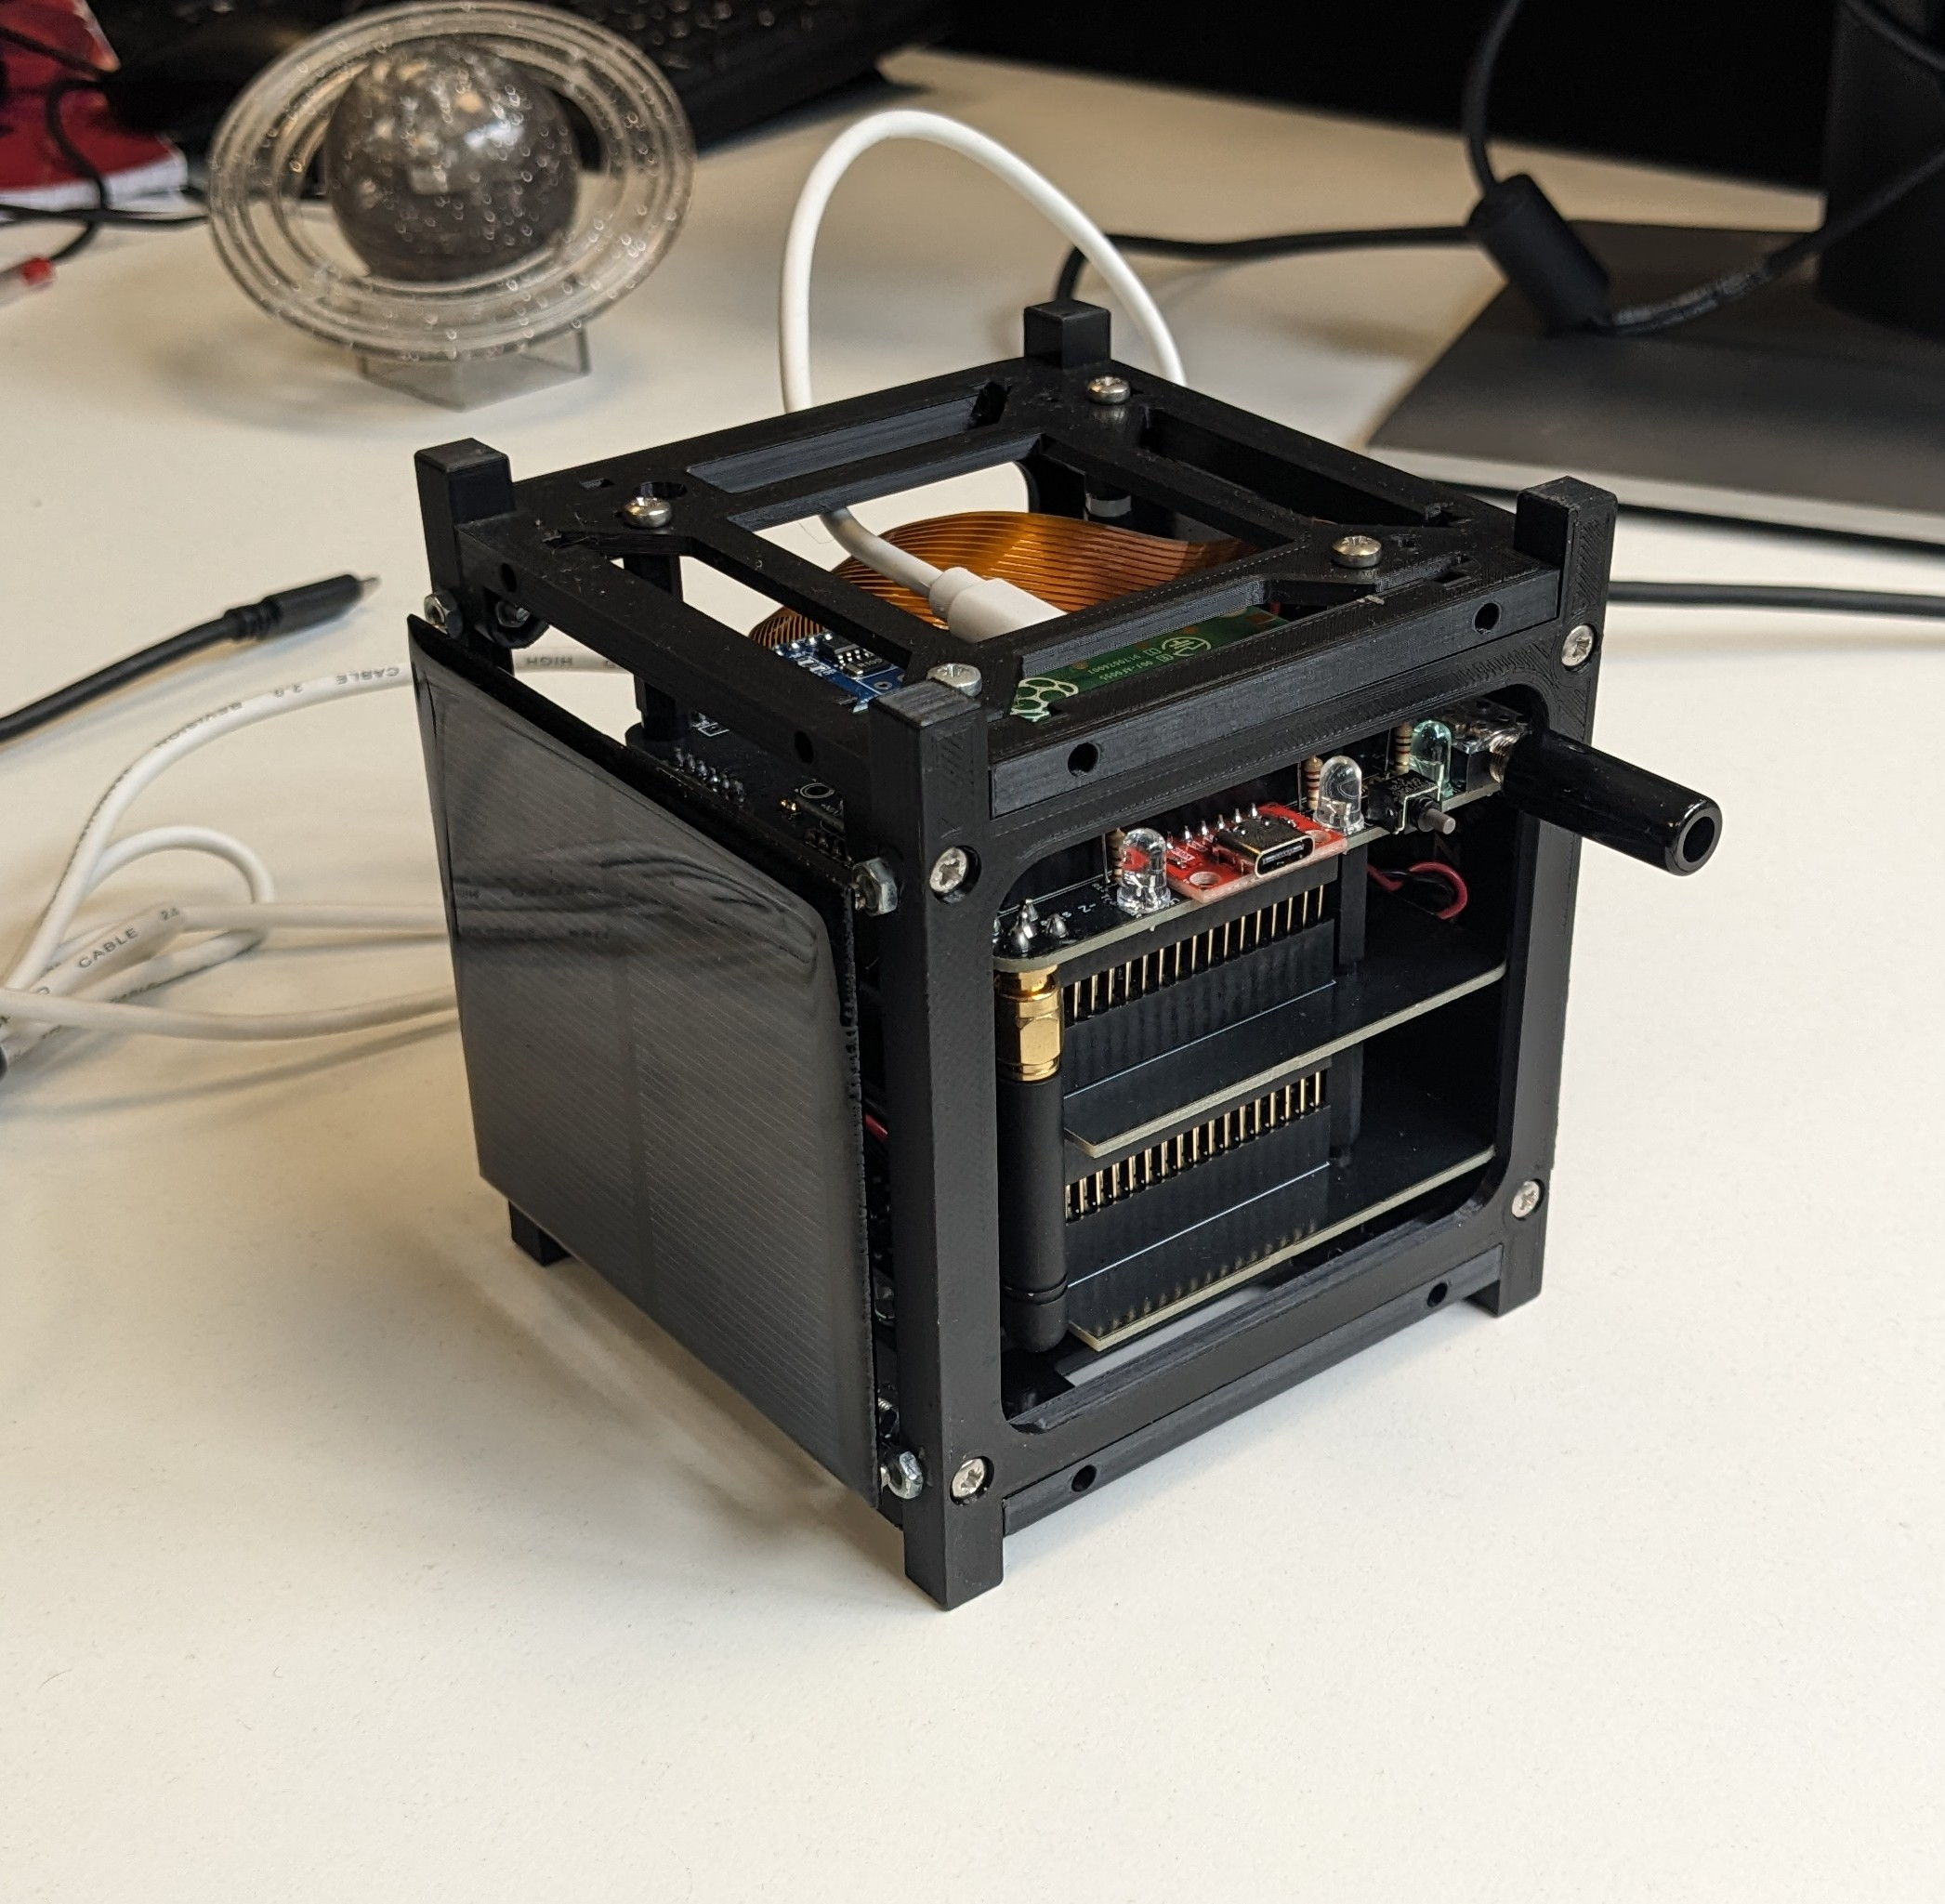
\includegraphics[width=0.7\linewidth, trim={2cm 2.5cm 0cm 0cm}, clip=true]{graphics/amsat_images/1000002586.jpg}
    \caption{A fully-assembled AMSAT, displaying the housing, a side-view of the PCB stack, and one of the side-mounted solar panels. A small RBF (``remove before flight'') pin can also be seen, which, when removed, triggers the RF mode and begins broadcasting telemetry packets over radio.}
    \label{fig:amsat-assembled}
\end{figure}


\section{Connecting to AMSATs}

\subsection{SSH \& WiFi}
\label{subsec:ssh}

Once you have assembled the AMSAT housing, we can now connect to the device. However, to connect to our AMSAT we have to do some configuration. Recall that when using platforms like GitHub we had the option use the secure shell or ssh protocol to clone a repo to our local machine. A more powerful use of the ssh protocol is that it can actually let us directly connect to a remote host and issue commands to the host as though it was our own local machine. In order to do this though we need to configure something called ``ssh keys'' on our local machine. On Windows machines this is not a very straight-forward process, but in our lab we will be using Linux machines with pre-configured keys so you will not need to be concerned about the details of this.\footnote{If you \textit{are} interested in the details, see the GitHub documentation about \href{https://docs.github.com/en/authentication/connecting-to-github-with-ssh/generating-a-new-ssh-key-and-adding-it-to-the-ssh-agent?platform=linux}{creating new ssh keys}.} We will assist you with the login details for these machines in the lab.

Just like with any other real-world communication, we need to know the \textit{address} of the machine we want to reach, and more importantly it needs to be a \textit{reachable} machine. Most often the address is an IP address or a \verb|<HOSTNAME>.local| address. When you open a terminal in Linux or Mac, the user and hostname are typically shown automatically; on Windows machines we can view the hostname in the System Settings. For the machine to be reachable it needs to either be on a local network or some remote network that is configured to allow external access. For our purposes, we will be using the AMSAT on a local network using either a wired USB connection or a Wi-Fi connection.

\newthought{USB Ethernet connection}

The first thing we need to do is use a micro-USB cable that allows data transmission as well as provides power. We will provide these in the lab, as well a cable tester you can use if you have any doubts. The micro-end of the cable goes into the middle input port on the Raspberry Pi (on the bottom of your AMSAT device), and you can plug the other end of your cable into the lab computer. When the AMSAT is powered on, you will see a blue LED turn on. This may take a few minutes to appear.

On the lab computer, the toolbar at the top right of your screen should show an internet connection icon; select this icon. In this window, if you see ``PCI Ethernet Connected`` then this tells you that your lab computer has an ethernet connection to the UCD network, so we want to leave that one alone. The AMSAT will show up under the ``USB Ethernet'' connection, and if the AMSAT is fully powered on you will see either ``USB Ethernet Connected'' or ``USB Ethernet Connecting''. Select the ``cog'' icon next to the UBS Ethernet option, alternatively, select the``Settings'' or ``Wired Settings'' option, as shown in Figure~\ref{fig:linux-network}. If you need further assistance finding these options (some version of Linux may display these things differently) let your instructor know. This will open the Network Settings dialogue.

\begin{marginfigure}
    \centering
    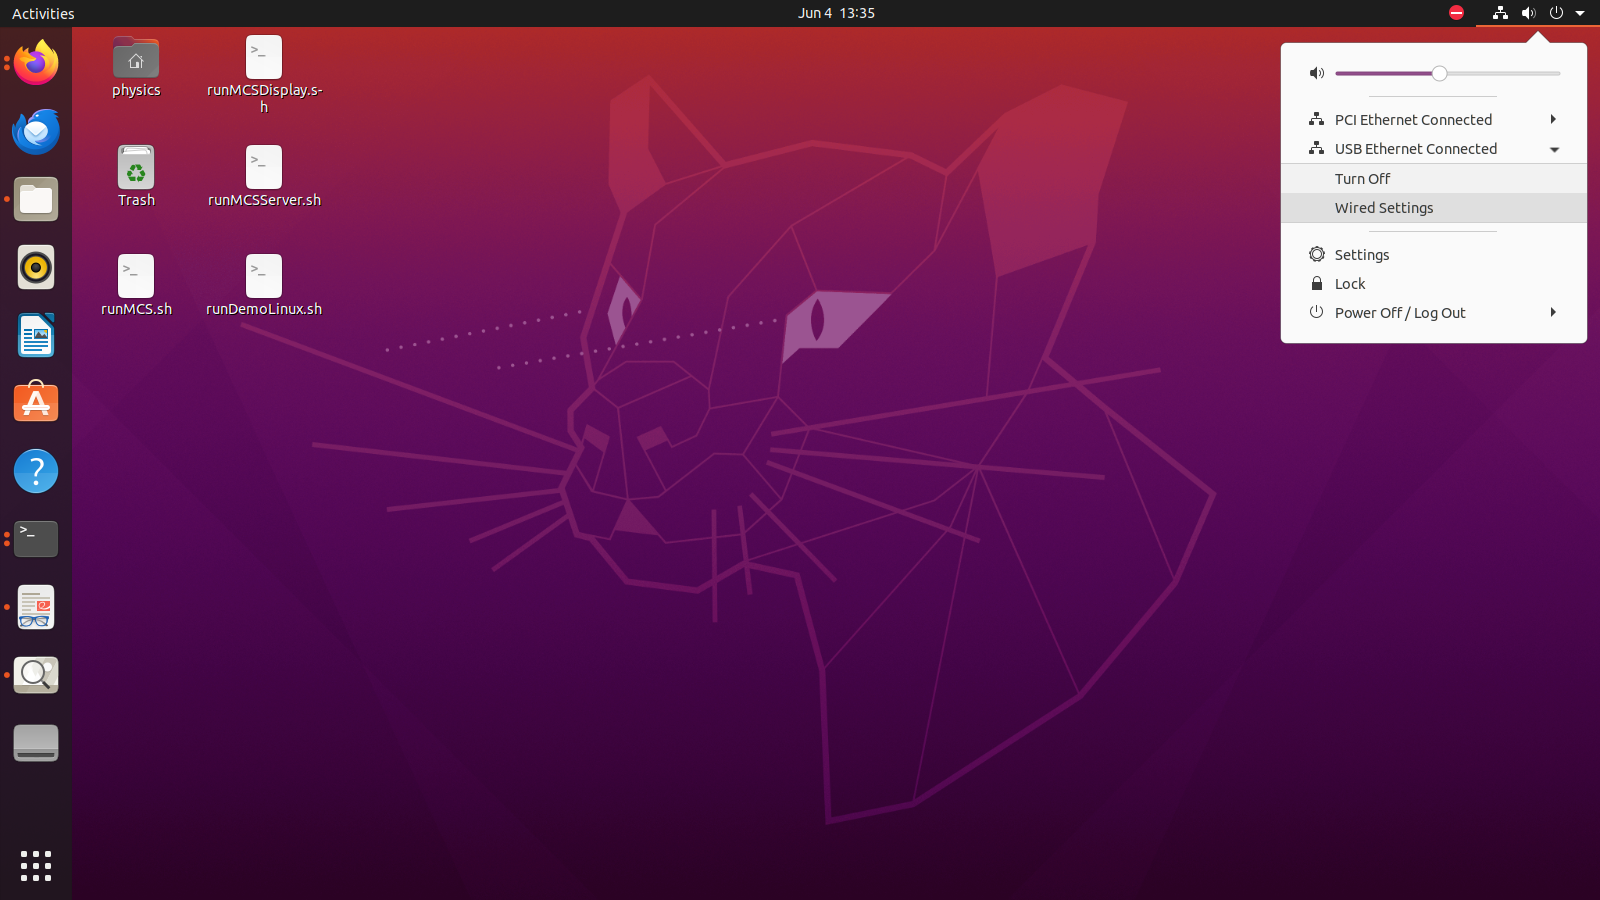
\includegraphics[width=0.9\linewidth, trim={44.5cm 19cm 0cm 0cm}, clip=true]{graphics/amsat_images/image02.png}
    \caption{The Linux network dialogue showing the different connections and options available.}
    \label{fig:linux-network}
\end{marginfigure}

By default, Linux will try to assign an IP address to your AMSAT automatically using DHCP. We do not want this. In the Network Settings window, select the wheel next to the USB Ethernet option and click the IPv4 tab. Make sure that the ``Link-Local Only'' option is selected in the IPv4 Method box (see Figure~\ref{fig:ipv4-config}). Click the IPv6 tab and make sure the IPv6 method is disabled. Save your connection settings and close the window. 

\begin{marginfigure}
    \centering
    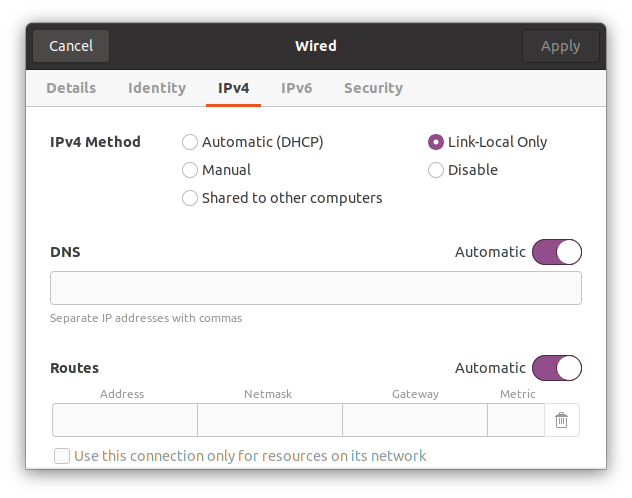
\includegraphics[width=0.95\linewidth]{graphics/amsat_images/figure04.png}
    \caption{The Wired Connection settings window. The IPv4 method is Link-Local Only, and IPv6 is disabled.}
    \label{fig:ipv4-config}
\end{marginfigure}
% \begin{lstlisting}[backgroundcolor = \color{lightgray},caption=Example code,label=fig:header]
% Here is some example code of how to set up conda
% \end{lstlisting}

\newthought{Finding the address}

Now that the AMSAT is configured as a link-local USB ethernet device, we can connect to it through the ssh protocol. Typically the address of a remote device has the format:

\begin{lstlisting}[backgroundcolor=\color{lightgray}]
# IP Address format
$ <USERNAME>@127.0.0.1
# .local address
$ <USERNAME>@<HOSTNAME>.local
\end{lstlisting}

For the AMSATs, the default user and host names are \verb|pi| and \verb|cubesatsim<N>.local|, where \verb|<N>| is the device number (see the sticker on your AMSAT box) and the default password is \verb|raspberry|. It is generally easier to know the hostname rather than the IP address, especially if the device is not in our local network. With this knowledge we can connect to the device pretty easily. You can click the terminal application icon on the left panel (it looks like \verb|>_|) or type \verb|ctrl+alt+t| to open it with the keyboard. For this example I am using \verb|cubesatsim1|, so in the terminal I will type:

\begin{lstlisting}[backgroundcolor=\color{lightgray}]
$ ssh -p 22 pi@cubesatsim1.local
\end{lstlisting}\marginnote[-7.6mm]{The \texttt{-p 22} tells the ssh client to connect over port number 22; this is the default port number used by ssh but we include it here just to be safe.}

If the connection was successful and this is the first time you have connected to the device, you will be shown a warning message like the one below with a key fingerprint and asked if you want to continue with the connection. We can type \verb|yes| because we know this is a trusted device, and then enter the default password for the AMSAT as noted above.

\begin{figure*}[h]
\begin{lstlisting}[backgroundcolor=\color{lightgray}, breaklines=true]
The authenticity of host 'cubesatsim1.local (<IP_ADDRESS>) can't be established.
ECDSA key fingerprint is SHA256:<SOME_STRING>.
Are you sure you want to continue connecting (yes/no.[fingerprint])?
\end{lstlisting}
\end{figure*}



\newthought{Communicating with the AMSAT}

All going well you are now connected to the AMSAT and your terminal should show \verb|pi@cubesatsim<N>:~$|. Since this is a terminal interface and not the more familiar graphical user interface with clickable folders, we have to use text commands to navigate and display information. You have seen some of these already with the Git commands; you are encouraged to explore \href{https://gist.github.com/bradtraversy/cc180de0edee05075a6139e42d5f28ce}{this GitHub page} which has a nice summary of the most common commands. Use the \verb|ls| and \verb|cd| commands to navigate around a bit and get more accustomed to the AMSAT directory structure.

\newthought{WiFi Connection}

To be written. For this one Andrew will need to set up the WiFi hotspot (which does not connect to the internet) so the students can connect over that. Necessary for the exercises with rotation!

\section{Reading sensors}

Because the AMSAT is ultimately a simulator, we can use it to gain familiarity with same of the basic functionalities of typical satellite subsystems. There are three sensor modules we will be working with on these devices.

\begin{itemize}
    \item the \textbf{BME280} -- measures temperature, pressure, and humidity;
    \item the \textbf{INA219} -- a power monitor which measures voltage and current;
    \item the \textbf{MPU6050} -- a combined accelerometer and gyroscope which measures motion in 6 axes
\end{itemize}

Provided with the AMSAT are two programs that allow us to access these measurements, and we will use a combination of Python and Linux commands to extract, save, and analyze the output.
Before we explore how to use these programs, we should first distinguish between two important types of programs, and understand how to run them in on Unix-like systems.

% \begin{itemize}
    % \item 
\textbf{Pre-compiled binaries} (like \verb|telem| and \verb|cubesatsim|) are stand-alone ``executables'' or ``binaries'' -- that is, they are ready to run on their own without any need for an interpreter to translate the code into a language the computer can understand. These can be run simply with:\marginnote{The ``dot-slash'' (\texttt{./}) is very important here; see the \href{https://www.linfo.org/dot_slash.html}{Linux Information Project page} for detailed discussion.}
\begin{lstlisting}[backgroundcolor=\color{lightgray}, language=Bash]
$ ./PROG_NAME
\end{lstlisting}

\textbf{Scripts} (like the Python files you will write) on the other hand are not stand-alone and these \textit{do} require an interpreter -- for example, with a Python script the computer needs to use the Python interpreter in order to read and understand our code. These can be run with:
\begin{lstlisting}[backgroundcolor=\color{lightgray}]
$ python SCRIPT_NAME.py
\end{lstlisting}
% \end{itemize}

% But first we will explore the basic functionality from the command line.

% \newthought{Connect the AMSAT} to the lab computer as discussed above. In the command line terminal, establish an ssh connection with the AMSAT and navigate to the \verb|CubeSatSim| directory. 


% \textbf{TODO: Move these next two paragraphs to a Jupyter Notebook?}
% Now that we understand these two file types, connect your AMSAT to the lab computer as discussed above and use the terminal to establish an ssh connection. Navigate to the \verb|CubeSatSim| directory (upper-case absolutely matters here) and run the \verb|telem| binary. You can copy and paste this output to your own text file or write it out yourself; either way, understanding the structure of this output is important. Next, do the same for the \verb|cubesatsim| binary. Note that you will need to let this program run for at least a few minutes.

% You will notice that the \verb|telem| output is easy to copy because it is a simple one-off program. The \verb|cubesatsim| output will keep going until we tell it to stop. Can you think of any benefits or drawbacks to these two approaches? Perhaps the most difficult thing here in terms of data analysis is copying the output: in both programs the output is printed to the screen, not a file, and while it is simple enough to copy and paste short pieces of output, if a program runs in a loop for an extended period of time the output will grow until it is unmanageable with the copy and paste method.

\newthought{Capturing Output}
% TO BE WRITTEN: Discuss capturing output streams, and segue into why we like using Python for this.

Before we discuss how to acquire data, we need to understand how computer programs communicate with their environments. This communication occurs over channels we call ``standard streams'', and there are three of these: \textbf{standard input} (\texttt{stdin}), \textbf{standard output} (\texttt{stdout}), and \textbf{standard error} (\texttt{stderr}). A visual schematic is shown in Figure~\ref{fig:iostreams}. We will spare the longer discussion on exactly what these things are, but for our purposes it's good enough to understand that on Unix-based machines the communication streams can be redirected and captured via the command line. 
\begin{marginfigure}
    \centering
    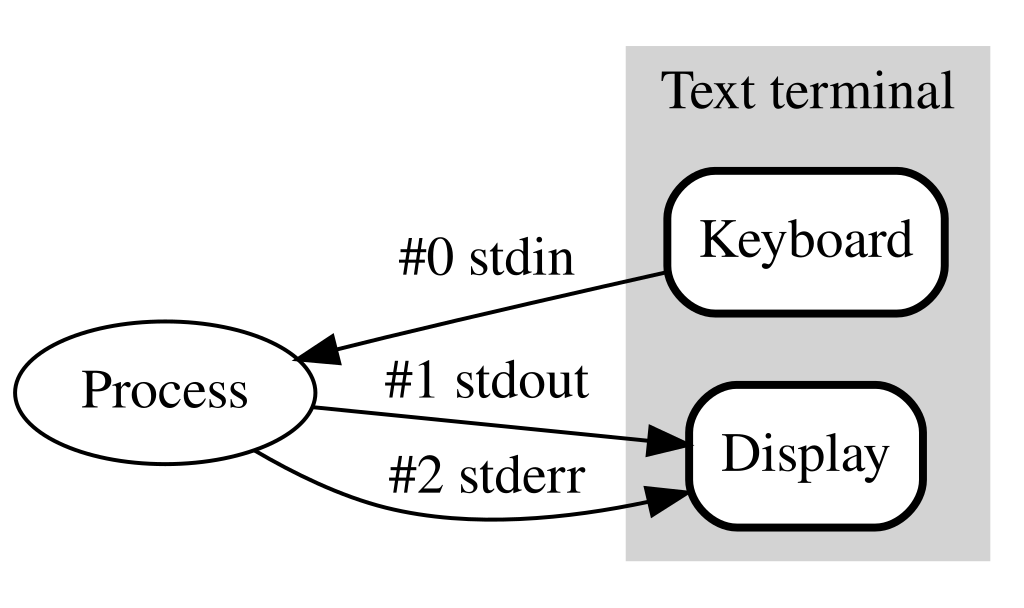
\includegraphics[width=\linewidth]{graphics/amsat_images/image05.png}
    \caption{A schematic of standard communication streams. you can read more about \href{https://www.linfo.org/standard_input.html}{standard input} and \href{https://www.linfo.org/standard_output.html}{standard output} if you are interested. Figure public domain courtesy of Wikipedia.}
    \label{fig:iostreams}
\end{marginfigure}

%Obviously sending a keyboard command would be considered as the \texttt{stdin} stream; the computer would then produce and output stream which you would see on your terminal. The \texttt{stdout} stream is where 


If I want to capture all of the output from a program and save it to a file, the most efficient way to do it is to tell the program to direct its output streams to a file. We can do this easily:
\begin{lstlisting}[backgroundcolor=\color{lightgray}, breaklines=true, language=Bash]
$ ./PROG_NAME > FILENAME
\end{lstlisting}
\noindent The \texttt{>} symbol tells the program to send the \verb|stdout| stream to \texttt{FILENAME}. Take care with this though because if \texttt{FILENAME} already exists, this will completely overwrite everything in that file. If we want to append to an already existing file, we use the \texttt{>>} operator:
\begin{lstlisting}[backgroundcolor=\color{lightgray}, breaklines=true]
$ ./PROG_NAME >> FILENAME
\end{lstlisting}
\noindent If the program prints both the \verb|stdout| and \verb|stderr| streams, we might want to capture both. We can do this in one of two ways: redirect both streams to the same file, or redirect each stream to its own file. 
\begin{lstlisting}[backgroundcolor=\color{lightgray}, breaklines=true]
# Send both streams to one file
$ ./PROGNAME &> FILE
# Send each stream to separate files
$ ./PROGNAME > FILE1 2> FILE2
\end{lstlisting}

% \textbf{TODO: Move some of this to a notebook?}
% \begin{tcolorbox}[sharp corners=all, colback=white!75!green, title=Try it Yourself]
% Complete Exercise $1$ in the ``lab1-amsat.introduction.ipynb'' Jupyter notebook.

% \end{tcolorbox} 

Note that the files to which you save your output will be on the AMSAT, not your lab machine. To move them to the lab machine we can use the \href{https://www.ssh.com/academy/ssh/sftp-ssh-file-transfer-protocol}{SSH file transfer protocol} or \verb|sftp|. Similar to the \verb|ssh| command we need to note the address and location of the file we want on the remote machine, and the location of where we want the move the file on our local machine. The syntax is simple:
\begin{lstlisting}[backgroundcolor=\color{lightgray}, breaklines=true]
$ sftp USER@REMOTE:PATH/TO/SOURCE /PATH/TO/DESTINATION
\end{lstlisting}
Let us assume we saved the output of \verb|cubesatsim| to a file called \verb|output.txt| in the \verb|CubeSatSim| directory, and we want to move this file to the \verb|Documents/AMSAT/| folder on our lab computer.
\begin{lstlisting}[backgroundcolor=\color{lightgray}, breaklines=true]
$ sftp pi@cubesatsim1.local:CubeSatSim/output.txt ~/Documents/AMSAT/
\end{lstlisting}
If we have typed everything correctly we will be prompted for the AMSAT password and the file will be copied to our \verb|AMSAT| folder. Try this yourself, replacing \verb|output.txt| with whatever filename you chose when using the \verb|./cubesatsim &> FILE| command.

The next issue we face is parsing this data. The AMSAT programs produce (somewhat) human-readable data, but we will find that we cannot simply load our files into, say, Excel, because they are not in a machine-readable (i.e. structured data) format. The solution to this is straight-forward but a bit tedious: at its most simple, we search for a pattern in a string, e.g. 
\begin{lstlisting}[backgroundcolor=\color{lightgray}, breaklines=true, language=Python, showstringspaces=false]
if "Some string" in line_of_text:
    # operate on that line
\end{lstlisting}

\noindent and carry on. A more advanced but rigorous approach is to use 
\textbf{regex} or \href{https://www.gnu.org/software/gnulib/manual/html_node/Regular-expressions.html}{``regular expression'' matching} to search the data and extract the pieces that we need.\footnote{The Python \texttt{re} module is excellent for this; however it is a more esoteric approach than the simpler string method.} This is essentially like an automated \verb|ctrl+f| in programming form. Whichever method we opt to use, we need to understand how the data is presented, hence the importance of examining the output of the programs before we develop a plan to parse it. We will cover this in more detail in the AMSAT practicals.

% Fortunately we have simplified this process for you. On your lab machine you will find the script \verb|parse_cubesatsim_output.sh| in the \texttt{AMSAT} directory. You are welcome to open this file in a text editor to explore how its written, but for our purposes it will be sufficient to simply execute the script. It is important to note though that this script requires a data file that you want to parse, so make sure you have successfully copied the data file from the AMSAT. To run this script, open a terminal, make sure you are in the \verb|AMSAT| directory, and type:
% \begin{lstlisting}[backgroundcolor=\color{lightgray}, breaklines=true]
% $ ./parse_cubesatsim_output.sh FILE
% \end{lstlisting}
% \noindent replacing \verb|FILE| with whatever filename you chose for your data. This will parse the file, extract the sensor data, and save the data to two new files: \verb|bme280_data.csv| and \verb|mpu6050_data.csv|. Finally you are ready to do some data analysis.
% \begin{itemize}
%     \item 
%         \textbf{Pre-compiled binaries} (like \verb|telem| are standalone executables and can be run simply with:
%         \begin{lstlisting}[backgroundcolor=\color{lightgray}]
%         $ ./<FILE_NAME>
%         \end{lstlisting}
%     \item
%         \textbf{Scripts} (like Python files) require an interpreter, which must be called first:
%         \begin{lstlisting}[backgroundcolor=\color{lightgray}]
%         $ python <SCRIPT_NAME>.py
%         \end{lstlisting}
% \end{itemize}

% The \verb|telem| and \verb|cubesatsim| tools are binaries -- that is, they are ready to run on their own without any need for an interpreter to translate the code into something the computer can understand. Scripts, on the other hand, are not stand-alone and these do require an interpreter -- when we write code in Python, the computer needs to use the Python interpreter to understand what our code means. 
% \begin{lstlisting}[backgroundcolor=\color{lightgray}]
% # Method 1
% $ ./<SCRIPT_NAME>
% # Method 2
% \end{lstlisting}

% It is important to note the \verb|./| (``dot-slash'') in front of the script name. 



\section{Exercises}

In our AMSAT practicals, we will be working through several Jupyter Notebooks, the first notebook of which will provide you with an introduction to the AMSAT and how to interface with it using Python. You will additionally perform the following experiments:

\begin{tcolorbox}[sharp corners=all, colback=white!75!green]
%[width=\linewidth, sharp corners=all, colback=white!95!black]
\begin{itemize}   
\item Placing the AMSAT on a turntable, record the voltage produced by the solar panels as a function of time. Exporting this data to a Jupyter notebook, determine the angular rotation rate of the AMSAT. The best way of doing this will be through a Fourier analysis of the voltage data; scipy and astropy contain many useful libraries for this.
\item Determine the angular acceleration using the onboard accelerometer. How does this compare to what you indirectly infer from the solar panel voltages, and what can you say about the accuracy of the two methods, and the tolerance of the turntables?
\item How does the degradation of solar panels affect the output voltage? You can explore this by covering part of the panels with paper and tape (do not apply tape directly to the panel surface) or alternatively by carefully coating one of the panels with chalk dust. How does the voltage and current change with fraction of the panel that is available?
\item When you query a sensor over ssh (perhaps through a Jupyter notebook) it will take a finite time to execute. What is the delay introduced by the groundstation (i.e. your computer), compared to on-board processing? Is this constant, or does this change if the AMSAT is trying to do several things at once? You can explore this with the \verb|time| command either from the terminal or through Python.
\end{itemize}

\end{tcolorbox} 


Each of the exercises above should be answered with a one page write-up, including where necessary any plots and figures. Focus on results and discussion rather than method or background.




%\chapter{Appendix: FAQ}

%\begin{itemize}

%\item Q: When I subtract two numpy arrays from each other I get strange numbers I don't expect like 65,536

%A: Look at what the data type of your numpy arrays is. Often, if you read in FITS files from the CCD they will be stored as unsigned 16-bit integers (``uint16''). These can contain any integer between 0 and $2^{16}-1$. However, if you subtract or add two arrays together and the result is larger than this (or negative) you will get strange results. The solution is to first change the dtype to int32 (or a float).

%\end{itemize}

%\chapter{Appendix: Sigma clipping}
%\label{ch:sigma}

%Suppose you asked a fellow student to measure the height of 10 people on campus for you. She returned with the following measurements:

%\begin{center}
%\begin{tabular}{| c| c| c |c|}
%\hline
%Person 1 &  1.82~m	& Person 6  & 1.76~m \\ 
%\hline
%Person 2 &  1.70~m	& Person 7  & 2.35~m \\ 
%\hline
%Person 3 &  1.75~m 	& Person 8  & 1.77~m \\ 
%\hline
%Person 4 &  1.80~m	& Person 9  & 1.81~m \\ 
%\hline
%Person 5 &  1.77~m	& Person 10 & 1.74~m \\ 
%\hline
%\end{tabular}
%\end{center}

%If we simply average all ten measurements, then we find an average height of 1.83~m. However, we can see that nine people are shorter than this average, and in fact the reason the average is so high is because of Person 7, who is 2.35~m tall.

%Now, it is possible that one of the people your fellow student measured was exceptionally tall. It is also possible that she made a measurement error, or a mistake recording the value. One may be tempted to arbitrarily remove this data point and recalculate the average, but this is not good practice.

%However, we can use a more rigorous argument to remove this outlying point. If we calculate the standard deviation of the measurements above, we find that Person 7 lies 2.8$\sigma$ from the mean. Let's assume that heights are normally distributed (this is probably reasonable for many things we measure). What is the probability that we would have a 2.8$\sigma$ outlier?

%From Fig. \ref{fig:gauss} we can see that there is about a 1 in 200 chance of finding a 2.8$\sigma$ outlier by chance. Given that we have only measured the heights of 10 people, it seems unlikely that this would occur. If on this basis we remove Person 7, we find that the average height decreases to 1.79$\pm$0.06~m, and everyone in our sample now has a height $<2\sigma$ from the new mean.

%\begin{figure}%
%  \includegraphics[width=\linewidth]{gaussian}
%  \caption{The percentage of normally distributed samples that are expected to be within 1, 2 or 3$\sigma$ of the mean.}
%  \label{fig:gauss}
%\end{figure}


%What we have just done is often referred to {\it sigma clipping}. To sigma clip a set of measurements, the necessary steps are: 
%\begin{enumerate}
%\item Calculate mean and standard deviation $\sigma$.
%\item Calculate how many $\sigma$ from the mean is each individual measurement.
%\item Remove any measurements that are more than $N \sigma$ from the mean (where $N$ is some threshold you have chosen).
%\item Repeat steps 1-3 until no more points are removed (or you have reached some pre-defined number of iterations).
%\end{enumerate}

%Some important caveats apply. Firstly, one is assuming that the data is normally distributed. This may not be the case, in which case sigma clipping will not necessarily be appropriate. As always, plotting the distribution of measurements is advisable.

%Secondly, one should think about the size of the dataset, and what sigma threshold you will adopt. If you have a million measurements, then you should not be surprised to see one or two 5$\sigma$ outliers.

%Finally, we must always think about {\it why} we are doing some operation on our data. In astronomy, one may sigma clip to remove {\it cosmic rays} (pixels where a charged particle has impacted the CCD). In this case, we have a solid reason to remove outliers, however, we should still note that this has been done when writing up our analysis.

%\chapter{Example Jupyter Notebook}
%\label{ch:example}

%This code shows an example of how you would read in some FITS files if you wanted to explore the dark current as a function of temperature. This is slightly different to what you need do in this experiment, but should help you get started with some of the fundamentals such as reading, manipulating and plotting FITS files.

%Please note that the error bars on the plot of counts versus CCD temperature appear too large, and you should think about why this is.

%\includepdf[
    %% Include all pages of the PDF
%    pages=-,
%    frame,
%    scale=0.85,
%    trim=10mm 10mm 10mm 10mm,
    %% make this page have the usual page style
    %% (you can change it to plain etc). By default pdfpages
    %% sets the pagecommand to \pagestyle{empty}
%    pagecommand={\pagestyle{headings}},  
    %% Add a "section" entry to the ToC with the heading
    %% "Quilling Shapes" and the label "sec:shapes"
%    addtotoc={1,section,1,Quilling Shapes,sec:shapes}]
%% The pdf file itself
%{analysis3.pdf}


\backmatter

%\bibliography{sample-handout}
%\bibliographystyle{plainnat}


%\printindex

\end{document}

